\documentclass[10]{article}
%\documentclass[11pt]{book}
\usepackage{hyperref}
\usepackage{amsfonts,amssymb,amsmath,amsthm,cite}
\usepackage{graphicx}
\usepackage[toc,page]{appendix}
\usepackage{nicefrac}
%% \usepackage[francais]{babel}
\usepackage[applemac]{inputenc}
\usepackage{amssymb, euscript}
\usepackage[matrix,arrow,curve]{xy}
\usepackage{graphicx}
\usepackage{tabularx}
\usepackage{float}
\usepackage{tikz}
\usepackage{slashed}
\usepackage{mathrsfs}
\usepackage{multirow}

%\usepackage{mathtools}

\usetikzlibrary{matrix}

\usepackage{siunitx}

\usepackage{lmodern}
\usepackage[T1]{fontenc}
\usepackage[babel=true]{microtype}


\usepackage{amsfonts,cite}
\usepackage{graphicx}

%% \usepackage[francais]{babel}
\usepackage[applemac]{inputenc}


\usepackage[sc]{mathpazo}
\usepackage{environ}

\linespread{1.05}         % Palatino needs more leading (space between lines)


%\usepackage[usenames]{color}



\DeclareFontFamily{T1}{pzc}{}
\DeclareFontShape{T1}{pzc}{m}{it}{1.8 <-> pzcmi8t}{}
\DeclareMathAlphabet{\mathpzc}{T1}{pzc}{m}{it}
% the command for it is \mathpzc

\textwidth=140mm


% % % % % % % % % % % % % % % % % % % %
\theoremstyle{plain}
\newtheorem{prop}{Proposition}[section]
\newtheorem{prdf}[prop]{Proposition and Definition}
\newtheorem{lem}[prop]{Lemma}%[section]
\newtheorem{cor}[prop]{Corollary}%[section]
\newtheorem{thm}[prop]{Theorem}%[section]
\newtheorem{theorem}[prop]{Theorem}
\newtheorem{lemma}[prop]{Lemma}
\newtheorem{proposition}[prop]{Proposition}
\newtheorem{corollary}[prop]{Corollary}
\newtheorem{statement}[prop]{Statement}

\theoremstyle{definition}
\newtheorem{defn}[prop]{Definition}%[section]
\newtheorem{cordefn}[prop]{Corollary and Definition}%[section]
\newtheorem{empt}[prop]{}%[section]
\newtheorem{exm}[prop]{Example}%[section]
\newtheorem{rem}[prop]{Remark}%[section]
\newtheorem{prob}[prop]{Problem}
\newtheorem{conj}{Conjecture}       %% Hypothesis 1
\newtheorem{cond}{Condition}        %% Condition 1
%\newtheorem{axiom}[thm]{Axiom}           %% Axiom 1 modified
\newtheorem{fact}[prop]{Fact}
\newtheorem{ques}{Question}         %% Question 1
\newtheorem{answ}{Answer}           %% Answer 1
\newtheorem{notn}{Notation}        %% Notations are not numbered

\theoremstyle{definition}
\newtheorem{notation}[prop]{Notation}
\newtheorem{definition}[prop]{Definition}
\newtheorem{example}[prop]{Example}
\newtheorem{exercise}[prop]{Exercise}
\newtheorem{conclusion}[prop]{Conclusion}
\newtheorem{conjecture}[prop]{Conjecture}
\newtheorem{criterion}[prop]{Criterion}
\newtheorem{summary}[prop]{Summary}
\newtheorem{axiom}[prop]{Axiom}
\newtheorem{problem}[prop]{Problem}
%\theoremstyle{remark}
\newtheorem{remark}[prop]{Remark}

\numberwithin{equation}{section}
\newtheorem*{claim}{Claim}
\DeclareMathOperator{\Dom}{Dom}              %% domain of an operator
\newcommand{\Dslash}{{D\mkern-11.5mu/\,}}    %% Dirac operator


%\newcommand\myeq{\stackrel{\mathclap{\normalfont\mbox{def}}}{=}}
\newcommand{\nor}[1]{\left\Vert #1\right\Vert}    %\nor{x}=||x||
\newcommand{\vertiii}[1]{{\left\vert\kern-0.25ex\left\vert\kern-0.25ex\left\vert #1
		\right\vert\kern-0.25ex\right\vert\kern-0.25ex\right\vert}}
\newcommand{\Ga}{\Gamma}  
\newcommand{\coker}{\mathrm{coker}}                   %% short for  \Gamma
\newcommand{\Coo}{C^\infty}                  %% smooth functions
% % % % % % % % % % % % % % % % % % % %


\usepackage[sc]{mathpazo}
\linespread{1.05}         % Palatino needs more leading (space between lines)

\newbox\ncintdbox \newbox\ncinttbox %% noncommutative integral symbols
\setbox0=\hbox{$-$} \setbox2=\hbox{$\displaystyle\int$}
\setbox\ncintdbox=\hbox{\rlap{\hbox
		to \wd2{\hskip-.125em \box2\relax\hfil}}\box0\kern.1em}
\setbox0=\hbox{$\vcenter{\hrule width 4pt}$}
\setbox2=\hbox{$\textstyle\int$} \setbox\ncinttbox=\hbox{\rlap{\hbox
		to \wd2{\hskip-.175em \box2\relax\hfil}}\box0\kern.1em}

\newcommand{\ncint}{\mathop{\mathchoice{\copy\ncintdbox}%
		{\copy\ncinttbox}{\copy\ncinttbox}%
		{\copy\ncinttbox}}\nolimits}  %% NC integral

%%% Repeated relations:
\newcommand{\xyx}{\times\cdots\times}      %% repeated product
\newcommand{\opyop}{\oplus\cdots\oplus}    %% repeated direct sum
\newcommand{\oxyox}{\otimes\cdots\otimes}  %% repeated tensor product
\newcommand{\wyw}{\wedge\cdots\wedge}      %% repeated exterior product
\newcommand{\subysub}{\subset\hdots\subset}      %% repeated subset
\newcommand{\supysup}{\supset\hdots\supset}      %% repeated supset
\newcommand{\rep}{\mathfrak{rep}}
\newcommand{\lift}{\mathfrak{lift}}
\newcommand{\desc}{\mathfrak{desc}}
%%% Roman letters:
\newcommand{\id}{\mathrm{id}}                %% identity map
\newcommand{\Id}{\mathrm{Id}}                %% identity map
\newcommand{\pt}{\mathrm{pt}}                %% a point
\newcommand{\const}{\mathrm{const}}          %% a constant
\newcommand{\codim}{\mathrm{codim}}          %% codimension
\newcommand{\cyc}{\mathrm{cyclic}}  %% cyclic sum
\renewcommand{\d}{\mathrm{d}}       %% commutative differential
\newcommand{\dR}{\mathrm{dR}}       %% de~Rham cohomology
\newcommand{\proj}{\mathrm{proj}}                %% a projection
\newcommand*{\braket}[2]{\langle#1 {,~} #2\rangle}% right inner products
\newcommand*{\lbraket}[2]{\langle\!\langle#1{\mid}#2\rangle\!\rangle}% left inner products

\newcommand*{\Mult}{\mathcal M}% multiplier algebra
\newcommand{\Lt}{\mathcal{L}}                 %%\newcommand{\unitsv}[1]{#1^{(0)}}

\newcommand{\A}{\mathcal{A}}                 %%\newcommand{\unitsv}[1]{#1^{(0)}}
\newcommand{\units}{G^{(0)}}
\newcommand{\haars}{\{\lambda^{u}\}_{u\in\units}}
\newcommand{\shaars}{\{\lambda_{u}\}_{u\in\units}}
\newcommand{\haarsv}[2]{\{\lambda^{#2}_{#1}\}_{#2\in\unitsv{#1}}}
\newcommand{\haarv}[2]{\lambda^{#2}_{#1}}

\renewcommand{\a}{\alpha}                    %% short for  \alphapha
\DeclareMathOperator{\ad}{ad}                %% infml adjoint repn
\newcommand{\as}{\quad\mbox{as}\enspace}     %% `as' with spacing
\newcommand{\Aun}{\widetilde{\mathcal{A}}}   %% unital algebra
\newcommand{\B}{\mathcal{B}}                 %% space of distributions
\newcommand{\E}{\mathcal{E}}                 %% space of distributions
\renewcommand{\b}{\beta}                     %% short for \beta
\newcommand{\braCket}[3]{\langle#1\mathbin|#2\mathbin|#3\rangle}
%\newcommand{\braket}[2]{\langle#1\mathbin|#2\rangle} %% <w|z>
\newcommand{\C}{\mathbb{C}}                  %% complex numbers
\newcommand{\CC}{\mathcal{C}}                %% space of distributions
\newcommand{\cc}{\mathbf{c}}                 %% Hochschild cycle
\DeclareMathOperator{\Cl}{C\ell}             %% Clifford algebra
\newcommand{\F}{\mathcal{F}}                 %% space of test functions
\newcommand{\G}{\mathcal{G}}                 %% 
\newcommand{\D}{\mathcal{D}}                 %% Moyal L^2-filtration
\renewcommand{\H}{\mathcal{H}}               %% Hilbert space
\newcommand{\half}{\tfrac{1}{2}}             %% small fraction  1/2
\newcommand{\hh}{\mathcal{H}}                %% Hilbert space
\newcommand{\hookto}{\hookrightarrow}        %% abbreviation
\newcommand{\Ht}{{\widetilde{\mathcal{H}}}}  %% Hilbert space of forms
\newcommand{\I}{\mathcal{I}}                 %% tracelike functions
\DeclareMathOperator{\Junk}{Junk}            %% the junk DGA ideal
\newcommand{\K}{\mathcal{K}}                 %% compact operators
\newcommand{\ket}[1]{|#1\rangle}             %% ket vector
\newcommand{\ketbra}[2]{|#1\rangle\langle#2|} %% rank one operator
\renewcommand{\L}{\mathcal{L}}               %% operator algebra
\newcommand{\La}{\Lambda}                    %% short for \Lambda
\newcommand{\la}{\lambda}                    %% short for \lambda
\newcommand{\lf}{L_f^\theta}                 %% left mult operator
\newcommand{\M}{\mathcal{M}}                 %% Moyal multplr algebra
\newcommand{\Lb}{\mathcal{L}}                 %% Moyal multplr algebra
\newcommand{\mm}{\mathcal{M}^\theta}
%\newcommand{{{\star_{\theta}}}{{\mathchoice{\mathbin{\;|\;ar_{_\theta}}}
			%            {\mathbin{\;|\;ar_{_\theta}}}           %% Moyal
			%            {{\;|\;ar_\theta}}{{\;|\;ar_\theta}}}}    %% product
	\newcommand{\N}{\mathbb{N}}                  %% nonnegative integers
	\newcommand{\NN}{\mathcal{N}}                %% a Moyal algebra
	\newcommand{\nb}{\nabla}                     %% gradient
	\newcommand{\Oh}{\mathcal{O}}                %% comm multiplier alg
	\newcommand{\om}{\omega}                     %% short for \omega
	\newcommand{\opp}{{\mathrm{op}}}             %% opposite algebra
	\newcommand{\ox}{\otimes}                    %% tensor product
	\newcommand{\eps}{\varepsilon}                    %% tensor product
	\newcommand{\otimesyox}{\otimes\cdots\otimes}    %% repeated tensor product
	\newcommand{\pa}{\partial}                   %% short for \partial
	\newcommand{\pd}[2]{\frac{\partial#1}{\partial#2}}%% partial derivative
	\newcommand{\piso}[1]{\lfloor#1\rfloor}      %% integer part
	\newcommand{\PsiDO}{\Psi~\mathrm{DO}}         %% pseudodiffl operators
	\newcommand{\Q}{\mathbb{Q}}                  %% rational numbers
	\newcommand{\R}{\mathbb{R}}                  %% real numbers
	\newcommand{\rdl}{R_\Dslash(\lambda)}        %% resolvent
	\newcommand{\roundbraket}[2]{(#1\mathbin|#2)} %% (w|z)
	\newcommand{\row}[3]{{#1}_{#2},\dots,{#1}_{#3}} %% list: a_1,...,a_n
	\newcommand{\sepword}[1]{\quad\mbox{#1}\quad} %% well-spaced words
	\newcommand{\set}[1]{\{\,#1\,\}}             %% set notation
	\newcommand{\Sf}{\mathbb{S}}                 %% sphere
	\newcommand{\uhor}[1]{\Omega^1_{hor}#1}
	\newcommand{\sco}[1]{{\sp{(#1)}}}
	\newcommand{\sw}[1]{{\sb{(#1)}}}
	\DeclareMathOperator{\spec}{sp}              %% spectrum
	\renewcommand{\SS}{\mathcal{S}}              %% Schwartz space
	\newcommand{\sss}{\mathcal{S}}               %% Schwartz space
	\DeclareMathOperator{\supp}{\mathfrak{supp}}            %% support
	\newcommand{\T}{\mathbb{T}}                  %% circle as a group
	\renewcommand{\th}{\theta}                   %% short for \theta
	\newcommand{\thalf}{\tfrac{1}{2}}            %% small* fraction 1/2
	\newcommand{\tihalf}{\tfrac{i}{2}}           %% small* fraction i/2
	\newcommand{\tpi}{{\tilde\pi}}               %% extended representation
	\DeclareMathOperator{\Tr}{Tr}                %% trace of operator
	\DeclareMathOperator{\tr}{tr}                %% trace of matrix
	\newcommand{\del}{\partial}                  %% short for  \partial
	\DeclareMathOperator{\tsum}{{\textstyle\sum}} %% small sum in display
	\newcommand{\V}{\mathcal{V}}                 %% test function space
	\newcommand{\vac}{\ket{0}}                   %% vacuum ket vector
	\newcommand{\vf}{\varphi}                    %% scalar field
	\newcommand{\w}{\wedge}                      %% exterior product
	\DeclareMathOperator{\wres}{wres}            %% density of Wresidue
	\newcommand{\x}{\times}                      %% cross
	\newcommand{\Z}{\mathbb{Z}}                  %% integers
	\newcommand{\7}{\dagger}                     %% short for + symbol
	\newcommand{\8}{\bullet}                     %% anonymous degree
	\renewcommand{\.}{\cdot}                     %% anonymous variable
	\renewcommand{\:}{\colon}                    %% colon in  f: A -> B
	
	%\newcommand{\sA}{\mathscr{A}}       %%
	\newcommand{\sA}{\mathcal{A}} 
	\newcommand{\sB}{\mathcal{B}}       %%
	\newcommand{\sC}{\mathcal{C}}       %%
	\newcommand{\sD}{\mathcal{D}}       %%
	\newcommand{\sE}{\mathcal{E}}       %%
	\newcommand{\sF}{\mathcal{F}}       %%
	\newcommand{\sG}{\mathcal{G}}       %%
	\newcommand{\sH}{\mathcal{H}}       %%
	\newcommand{\sI}{\mathcal{I}}       %%
	\newcommand{\sJ}{\mathcal{J}}       %%
	\newcommand{\sK}{\mathcal{K}}       %%
	\newcommand{\sL}{\mathcal{L}}       %%
	\newcommand{\sM}{\mathcal{M}}       %%
	\newcommand{\sN}{\mathcal{N}}       %%
	\newcommand{\sO}{\mathcal{O}}       %%
	\newcommand{\sP}{\mathcal{P}}       %%
	\newcommand{\sQ}{\mathcal{Q}}       %%
	\newcommand{\sR}{\mathcal{R}}       %%
	\newcommand{\sS}{\mathcal{S}}       %%
	\newcommand{\sT}{\mathcal{T}}       %%
	\newcommand{\sU}{\mathcal{U}}       %%
	\newcommand{\sV}{\mathcal{V}}       %%
	\newcommand{\sX}{\mathcal{X}}       %%
	\newcommand{\sY}{\mathcal{Y}}       %%
	\newcommand{\sZ}{\mathcal{Z}}       %%
	
	\newcommand{\Om}{\Omega}       %%
	
	
	\DeclareMathOperator{\ptr}{ptr}     %% Poisson trace
	\DeclareMathOperator{\Trw}{Tr_\omega} %% Dixmier trace
	\DeclareMathOperator{\vol}{Vol}     %% total volume
	\DeclareMathOperator{\Vol}{Vol}     %% total volume
	\DeclareMathOperator{\Area}{Area}   %% area of a surface
	\DeclareMathOperator{\Wres}{Wres}   %% (Wodzicki) residue
	
	\newcommand{\dd}[1]{\frac{\partial}{\partial#1}}   %% partial derivation
	\newcommand{\ddt}[1]{\frac{d}{d#1}}                %% derivative
	\newcommand{\inv}[1]{\frac{1}{#1}}                 %% inverse
	\newcommand{\sfrac}[2]{{\scriptstyle\frac{#1}{#2}}} %% tiny fraction
	
	\newcommand{\bA}{\mathbb{A}}       %%
	\newcommand{\bB}{\mathbb{B}}       %%
	\newcommand{\bC}{\mathbb{C}}       %%
	\newcommand{\bCP}{\mathbb{C}P}     %%
	\newcommand{\bD}{\mathbb{D}}       %%
	\newcommand{\bE}{\mathbb{E}}       %%
	\newcommand{\bF}{\mathbb{F}}       %%
	\newcommand{\bG}{\mathbb{G}}       %%
	\newcommand{\bH}{\mathbb{H}}       %%
	\newcommand{\bHP}{\mathbb{H}P}     %%
	\newcommand{\bI}{\mathbb{I}}       %%
	\newcommand{\bJ}{\mathbb{J}}       %%
	\newcommand{\bK}{\mathbb{K}}       %%
	\newcommand{\bL}{\mathbb{L}}       %%
	\newcommand{\bM}{\mathbb{M}}       %%
	\newcommand{\bN}{\mathbb{N}}       %%
	\newcommand{\bO}{\mathbb{O}}       %%
	\newcommand{\bOP}{\mathbb{O}P}     %%
	\newcommand{\bP}{\mathbb{P}}       %%
	\newcommand{\bQ}{\mathbb{Q}}       %%
	\newcommand{\bR}{\mathbb{R}}       %%
	\newcommand{\bRP}{\mathbb{R}P}     %%
	\newcommand{\bS}{\mathbb{S}}       %%
	\newcommand{\bT}{\mathbb{T}}       %%
	\newcommand{\bU}{\mathbb{U}}       %%
	\newcommand{\bV}{\mathbb{V}}       %%
	\newcommand{\bX}{\mathbb{X}}       %%
	\newcommand{\bY}{\mathbb{Y}}       %%
	\newcommand{\bZ}{\mathbb{Z}}       %%
	
	\newcommand{\bydef}{\stackrel{\mathrm{def}}{=}}          %% 
	\newcommand{\defeq}{\stackrel{\mathrm{def}}{=}}   
	
	
	
	\newcommand{\al}{\alpha}          %% short for  \alpha
	\newcommand{\bt}{\beta}           %% short for  \beta
	\newcommand{\Dl}{\Delta}          %% short for  \Delta
	\newcommand{\dl}{\delta}          %% short for  \delta
	\newcommand{\ga}{\gamma}          %% short for  \gamma
	\newcommand{\ka}{\kappa}          %% short for  \kappa
	\newcommand{\sg}{\sigma}          %% short for  \sigma
	\newcommand{\Sg}{\Sigma}          %% short for  \Sigma
	\newcommand{\Th}{\Theta}          %% short for  \Theta
	\renewcommand{\th}{\theta}        %% short for  \theta
	\newcommand{\vth}{\vartheta}      %% short for  \vartheta
	\newcommand{\ze}{\zeta}           %% short for  \zeta
	
	\DeclareMathOperator{\ord}{ord}     %% order of a PsiDO
	\DeclareMathOperator{\rank}{rank}   %% rank of a vector bundle
	\DeclareMathOperator{\sign}{sign}   %%
	\DeclareMathOperator{\sgn}{sgn}   %%
	\DeclareMathOperator{\chr}{char}   %%
	\DeclareMathOperator{\ev}{ev}       %% evaluation
	
	
	\newcommand{\Op}{\mathbf{Op}}
	\newcommand{\As}{\mathbf{As}}
	\newcommand{\Com}{\mathbf{Com}}
	\newcommand{\LLie}{\mathbf{Lie}}
	\newcommand{\Leib}{\mathbf{Leib}}
	\newcommand{\Zinb}{\mathbf{Zinb}}
	\newcommand{\Poiss}{\mathbf{Poiss}}
	
	\newcommand{\gX}{\mathfrak{X}}      %% vector fields
	\newcommand{\sol}{\mathfrak{so}}    %% special orthogonal Lie algebra
	\newcommand{\gm}{\mathfrak{m}}      %% maximal ideal
	
	
	\DeclareMathOperator{\Res}{Res}
	\DeclareMathOperator{\NCRes}{NCRes}
	\DeclareMathOperator{\Ind}{Ind}
	%% co/homology theories
	\DeclareMathOperator{\rH}{H}        %% any co/homology
	\DeclareMathOperator{\rC}{C}        %%  any co/chains
	\DeclareMathOperator{\rZ}{Z}        %% cycles
	\DeclareMathOperator{\rB}{B}        %% boundaries
	\DeclareMathOperator{\rF}{F}        %% filtration
	\DeclareMathOperator{\Gr}{gr}        %% associated graded object
	\DeclareMathOperator{\rHc}{H_{\mathrm{c}}}   %% co/homology with compact support
	\DeclareMathOperator{\drH}{H_{\mathrm{dR}}}  %% de Rham co/homology
	\DeclareMathOperator{\cechH}{\check{H}}    %% Cech co/homology
	\DeclareMathOperator{\rK}{K}        %% K-groups
	\DeclareMathOperator{\rKO}{KO}        %% real K-groups
	\DeclareMathOperator{\rKU}{KU}        %% unitary K-groups
	\DeclareMathOperator{\rKSp}{KSp}        %% symplectic K-groups
	\DeclareMathOperator{\rR}{R}        %% representation ring
	\DeclareMathOperator{\rI}{I}        %% augmentation ideal
	\DeclareMathOperator{\HH}{HH}       %% Hochschild co/homology
	\DeclareMathOperator{\HC}{HC}       %% cyclic co/homology
	\DeclareMathOperator{\HP}{HP}       %% periodic cyclic co/homology
	\DeclareMathOperator{\HN}{HN}       %% negative cyclic co/homology
	\DeclareMathOperator{\HL}{HL}       %% Leibniz co/homology
	\DeclareMathOperator{\KK}{KK}       %% KK-theory
	\DeclareMathOperator{\KKK}{\mathbf{KK}}       %% KK-theory as a category
	\DeclareMathOperator{\Ell}{Ell}       %% Abstract elliptic operators
	\DeclareMathOperator{\cd}{cd}       %% cohomological dimension
	\DeclareMathOperator{\spn}{span}       %% span
	\DeclareMathOperator{\linspan}{span} %% linear span (can't use \span)
	\newcommand{\blank}{-}   
	
	
	
	\newcommand{\twobytwo}[4]{\begin{pmatrix} #1 & #2 \\ #3 & #4 \end{pmatrix}}
	\newcommand{\CGq}[6]{C_q\!\begin{pmatrix}#1&#2&#3\\#4&#5&#6\end{pmatrix}}
	%% q-Clebsch--Gordan coefficients
	\newcommand{\cz}{{\bullet}}         %% anonymous degree
	\newcommand{\nic}{{\vphantom{\dagger}}} %% invisible dagger
	\newcommand{\ep}{{\dagger}}         %% abbreviation for + symbol
	\newcommand{\downto}{\downarrow}    %% right hand limit
	\newcommand{\isom}{\cong}          %% isomorphism
	\newcommand{\lt}{\triangleright}    %% a left action
	\newcommand{\otto}{\leftrightarrow} %% bijection
	\newcommand{\rt}{\triangleleft}     %% a right action
	\newcommand{\semi}{\rtimes}         %% crossed product
	\newcommand{\tensor}{\otimes}       %% tensor product
	\newcommand{\cotensor}{\square}       %% cotensor product
	\newcommand{\trans}{\pitchfork}     %% transverse
	\newcommand{\ul}{\underline}        %% for sheaves
	\newcommand{\upto}{\uparrow}        %% left hand limit
	\renewcommand{\:}{\colon}           %% colon in  f: A -> B
	\newcommand{\blt}{\ast}
	\newcommand{\Co}{C_{\bullet}}
	\newcommand{\cCo}{C^{\bullet}}
	\newcommand{\nbs}{\nabla^S}         %% spin connection
	\newcommand{\up}{{\mathord{\uparrow}}} %% `up' spinors
	\newcommand{\dn}{{\mathord{\downarrow}}} %% `down' spinors
	\newcommand{\updn}{{\mathord{\updownarrow}}} %% up or down
	
	%%% Bilinear enclosures:
	
	\newcommand{\bbraket}[2]{\langle\!\langle#1\stroke#2\rangle\!\rangle}
	%% <<w|z>>
	\newcommand{\bracket}[2]{\langle#1,\, #2\rangle} %% <w,z>
	\newcommand{\scalar}[2]{\langle#1,\,#2\rangle} %% <w,z>
	\newcommand{\poiss}[2]{\{#1,\,#2\}} %% {w,z}
	\newcommand{\dst}[2]{\langle#1,#2\rangle} %% distributions <u,\phi>
	\newcommand{\pairing}[2]{(#1\stroke #2)} %% right-linear pairing
	\def\<#1|#2>{\langle#1\stroke#2\rangle} %% \braket (Dirac notation)
	\def\?#1|#2?{\{#1\stroke#2\}}        %% left-linear pairing
	
	%%% Accent-like macros:
	
	\renewcommand{\Bar}[1]{\overline{#1}} %% closure operator
	\renewcommand{\Hat}[1]{\widehat{#1}}  %% short for \widehat
	\renewcommand{\Tilde}[1]{\widetilde{#1}} %% short for \widetilde
	
	
	\DeclareMathOperator{\bCl}{\bC l}   %% complex Clifford algebra
	
	%%% Small fractions in displays:
	
	\newcommand{\ihalf}{\tfrac{i}{2}}   %% small fraction  i/2
	\newcommand{\quarter}{\tfrac{1}{4}} %% small fraction  1/4
	\newcommand{\shalf}{{\scriptstyle\frac{1}{2}}}  %% tiny fraction  1/2
	\newcommand{\third}{\tfrac{1}{3}}   %% small fraction  1/3
	\newcommand{\ssesq}{{\scriptstyle\frac{3}{2}}} %% tiny fraction  3/2
	\newcommand{\sesq}{{\mathchoice{\tsesq}{\tsesq}{\ssesq}{\ssesq}}} %% 3/2
	\newcommand{\tsesq}{\tfrac{3}{2}}   %% small fraction  3/2
	
	
	%\newcommand\eqdef{\overset{\mathclap{\normalfont\mbox{def}}}{=}}
	\newcommand\eqdef{\overset{\mathrm{def}}{=}}
	
	
	%+++++++++++++++++++++++++++++++++++
	
	\newcommand{\word}[1]{\quad\text{#1}\enspace} %% well-spaced words
	\newcommand{\words}[1]{\quad\text{#1}\quad} %% better-spaced words
	\newcommand{\su}[1]{{\sp{[#1]}}}
	
	\def\<#1,#2>{\langle#1,#2\rangle}            %% bilinear pairing
	\def\ee_#1{e_{{\scriptscriptstyle#1}}}       %% basis projector
	\def\wick:#1:{\mathopen:#1\mathclose:}       %% Wick-ordered operator
	
	\newcommand{\opname}[1]{\mathop{\mathrm{#1}}\nolimits}
	
	\newcommand{\hideqed}{\renewcommand{\qed}{}} %% to suppress `\qed'
	
	
	%%%%%%%%%%%%%%%%%%%%%%%%%%%%%
	%% 2. Some internal machinery
	%%%%%%%%%%%%%%%%%%%%%%%%%%%%%
	
	\newbox\ncintdbox \newbox\ncinttbox %% noncommutative integral symbols
	\setbox0=\hbox{$-$}
	\setbox2=\hbox{$\displaystyle\int$}
	\setbox\ncintdbox=\hbox{\rlap{\hbox
			to \wd2{\box2\relax\hfil}}\box0\kern.1em}
	\setbox0=\hbox{$\vcenter{\hrule width 4pt}$}
	\setbox2=\hbox{$\textstyle\int$}
	\setbox\ncinttbox=\hbox{\rlap{\hbox
			to \wd2{\hskip-.05em\box2\relax\hfil}}\box0\kern.1em}
	
	\newcommand{\disp}{\displaystyle} %% short for  \displaystyle
	
	%\newcommand{\hideqed}{\renewcommand{\qed}{}} %% no `\qed' at end-proof
	
	\newcommand{\stroke}{\mathbin|}   %% (for `\bbraket' and such)
	\newcommand{\tribar}{|\mkern-2mu|\mkern-2mu|} %% norm bars: |||
	
	%%% Enclose one argument with delimiters:
	
	\newcommand{\bra}[1]{\langle{#1}\rvert} %% bra vector <w|
	\newcommand{\kett}[1]{\lvert#1\rangle\!\rangle} %% ket 2-vector |y>>
	\newcommand{\snorm}[1]{\mathopen{\tribar}{#1}%
		\mathclose{\tribar}}                 %% norm |||x|||
	
	
	\newcommand{\End}{\mathrm{End}}       %%
	\newcommand{\Ext}{\mathrm{Ext}}       %%
	\newcommand{\Hom}{\mathrm{Hom}}       %%
	\newcommand{\Mrt}{\mathrm{Mrt}}       %%
	\newcommand{\grad}{\mathrm{grad}}       %%
	\newcommand{\Spin}{\mathrm{Spin}}       %%
	\newcommand{\Ad}{\mathrm{Ad}}       %%
	\newcommand{\Pic}{\mathrm{Pic}}       %%
	\newcommand{\Aut}{\mathrm{Aut}}       %%
	\newcommand{\Inn}{\mathrm{Inn}}       %%
	\newcommand{\Out}{\mathrm{Out}}       %%
	\newcommand{\Homeo}{\mathrm{Homeo}}       %%
	\newcommand{\Diff}{\mathrm{Diff}}       %%
	\newcommand{\im}{\mathrm{im}}       %%
	
	
	\newcommand{\SO}{\mathrm{SO}}       %%
	\newcommand{\SU}{SU}       %%
	\newcommand{\gso}{\mathfrak{so}}    %% special orthogonal Lie algebra
	\newcommand{\gero}{\mathfrak{o}}    %% orthogonal Lie algebra
	\newcommand{\gspin}{\mathfrak{spin}} %% spin Lie algebra
	\newcommand{\gu}{\mathfrak{u}}      %% unitary Lie algebra
	\newcommand{\gsu}{\mathfrak{su}}    %% special unitary Lie algebra
	\newcommand{\gsl}{\mathfrak{sl}}    %% special linear Lie algebra
	\newcommand{\gsp}{\mathfrak{sp}}    %% symplectic linear Lie algebra
	
	%\newcommand{\bes}{\begin{equation}\begin{split}}
			%\newcommand{\ees}{\end{split}\end{equation}}
	%\NewEnviron{split.enviro}{%
		%	\begin{equation}\begin{split}
				%	\BODY
				%	\end{split}\end{equation}
		%$}
	\newenvironment{splitequation}{\begin{equation}\begin{split}}{\end{split}\end{equation}}
	
	%Begin equation split: Begin equation split = bes
	\newcommand{\bs}{\begin{split}}
		\newcommand{\es}{\end{split}}
	\newcommand{\be}{\begin{equation}}
		\renewcommand{\ee}{\end{equation}}
	\newcommand{\bea}{\begin{eqnarray}}
		\newcommand{\eea}{\end{eqnarray}}
	\newcommand{\bean}{\begin{eqnarray*}}
		\newcommand{\eean}{\end{eqnarray*}}
	\newcommand{\brray}{\begin{array}}
		\newcommand{\erray}{\end{array}}
	\newenvironment{equations}
	{\begin{equation}
			\begin{split}}
			{\end{split}
	\end{equation}}
	\newcommand{\Hsquare}{%
		\text{\fboxsep=-.2pt\fbox{\rule{0pt}{1ex}\rule{1ex}{0pt}}}%
	}
	
	\title{The Dixmier�Douady theory for $C^*$-algebras of foliations}
	
	\author
	{\textbf{Petr R. Ivankov*}\\
		e-mail: * monster.ivankov@gmail.com \\
	}
	
	\begin{document}

\maketitle  %\setlength{\parindent}{0pt}
\pagestyle{plain}


%\vspace{1 in}


%\noindent

\begin{abstract}
The Dixmier�Douady theory states some properties  of $C^*$-algebras having continuous trace. These algebras uniquely depend on the Dixmier�Douady invariant which is a cohomological cocycle. There are a natural pairings of both continuous trace $C^*$-algebras and their $K$-groups. We prove that there are similar ingredients for $C^*$-algebras of foliations, that is these algebras depend on cohomological cycle, also there are natural pairings of these  $C^*$-algebras and their cohomology groups.
\end{abstract}

\tableofcontents
%\end{abstract}

\section{Motivation}

\paragraph{}
The Dixmier�Douady theory yields  pairings of $C^*$-algebras (cf. Proposition \ref{ctr_d_prop}) and their $K$-groups (cf. Proposition \ref{ctr_cup_prop}).



\begin{proposition}\label{ctr_d_prop}\cite{cuntz_meyer_ros:bivariant}
	%Proposition 9.11 (P. Green [51,96,104]). 
	Let $\sX$ be a second-countable locally compact
	Hausdorff space, and let $A$ and $B$ be stable algebras of continuous trace over $\sX$.
	Then $A \times_\sX B$ is also a stable continuous-trace algebra over $\sX$, and the Dixmier�Douady class $\dl \left(A \otimes_\sX B \right)$  of $A \times_\sX B$ is given by $\dl(A) + \dl(B)$. The Dixmier�Douady class of the opposite algebra $A^{\mathrm{op}}$ is given by $\dl\left( A^{\mathrm{op}}\right)=$ - $\dl\left( A\right)$ , so that
	$A\times_\sX  A^{\mathrm{op}}= C_0\left(\sX, \K\right)$.
\end{proposition}
\begin{remark}\label{fam_rem}
The notation $A \times_\sX B$ means the following. For all $x\in \sX$ there are irreducible representations $\pi_x^A: A \to  B\left( \H_x\right)$ and $\pi_x^B: B \to  B\left( \H_x\right)$. Any pair $\left(a, b\right)\in A\times B$ yields a family 
\be\label{fam_eqn}
\left\{\pi_x^A\left(a \right) \otimes_\C \pi_x^B\left(b \right)\right\}_{x\in \sX} \in  \prod_{x\in \sX} \K\left(\H_x\otimes \H_x \right) 
\ee
The space $A \otimes_\sX B$ is a $\C$-subspace of $\prod_{x\in \sX} \K\left(\H_x\otimes \H_x \right)$  generated by given by \eqref{fam_eqn} elements.
\end{remark}
\begin{notation}\label{ctr_not}
	If $\sX$ is a locally compact Hausdorff space then we denote by $CT\left(\sX, \dl \right)$ the stable
	continuous-trace algebra  with Dixmier�Douady class $\delta \in \check{H}^3\left(\sX,\Z \right)$. From the Proposition \ref{ctr_d_prop} it follows that
	\be\label{bundle_prod_iso}
	CT\left(\sX, \dl \right)\times_\sX CT\left(\sX, \rho \right)\cong CT\left(\sX, \dl +\rho\right).
	\ee
\end{notation}
\begin{proposition}\label{ctr_cup_prop}\cite{cuntz_meyer_ros:bivariant}
	%Proposition 9.17.
	There is a natural homomorphisms
	\be\label{ka_eqn}
	K_\bullet\left( CT\left(\sX, \dl \right)\right)\otimes_\Z K_\bullet\left( CT\left(\sX, \rho \right)\right) \to K_\bullet\left( CT\left(\sX, \dl + \rho\right)\right),
	\ee
	where $K_\bullet\left( CT\left(\sX, \dl \right)\right)$ means $K$-theoretic groups of $C^*$-algebra $ CT\left(\sX, \dl \right)$ and $K^\bullet\left( \sX\right)$ means $K$-theoretic groups of the space $\sX$.
\end{proposition}
My article \cite{ivankov:grot_ca} contains an equation 
\be\label{ha_eqn}
\check{H}^\bullet\left(CT\left( \sX, \delta\right) , F \right) \otimes_{\check{H}^\bullet\left( \sX, F\right)  }\check{H}^\bullet\left(CT\left( \sX, \rho\right) , F \right) \to \check{H}^\bullet\left(CT\left( \sX, {\delta + \rho}\right) , F \right).
\ee
which is  an analog of the equation \eqref{ka_eqn}.


If $\G$ ia a topological groupoid and $\a \in H^2\left(\G, \T \right)$ is a cocycle then there is a $C^*$-algebra $C^*\left(\G, \a \right)$ (cf. \cite{renault:gropoid_ca}).  Foe any $\a, \bt \in H^2\left(\G, \T \right)$ we would like to find an isomorphism
\be\label{foli_prodp_eqn}
	C^*\left(\G, \a \right)\times_\sX C^*\left(\G, \bt \right)\cong C^*\left(\G, \a + \bt \right)
\ee
where $\sX$ is a spectrum of both $C^*\left(\G, \a \right)$ and $C^*\left(\G, \a \right)$, the product $	C^*\left(\G, \a \right)\times_\sX C^*\left(\G, \bt \right)$ is similar to the explained in the Remark \ref{fam_rem} one. The equation \eqref{foli_prodp_eqn} is an analog of the  \eqref{bundle_prod_iso} one. Also we would like find  a pairing
$$
\check{H}^\bullet\left( C^*\left(\G, \a \right) , F \right) \otimes_{\check{H}^\bullet\left( C^*\left(\G, 0 \right) , F \right) }\check{H}^\bullet\left( C^*\left(\G, \bt \right) , F \right) \to \check{H}^\bullet\left( C^*\left(\G, \a + \bt \right) , F \right)
$$
which is an analog of the given by the equations \eqref{ka_eqn}, \eqref{ha_eqn} ones.

\section{Pairings of  $C^*$-algebras of foliations}
groupoids of such spaces are Hausdorff.
\subsection{Reduced sheaf  of the foliation}
\begin{empt} \label{foli_sheaf_empt}
	Let $\sV \subset \G\left(M, \sF  \right)$ be an open subset. For any $x \in M$ denote by
	\be
	\begin{split}
		\ker_\sV \bydef \bigcap_{\substack{a \in \Ga_c\left(M, \Om^{1/2}\right) \\ \supp a \subset \sV} }\ker \rho_x\left( a\right),\\ 
		\im_\sV \bydef  \bigcup_{\substack{a \in  \Ga_c\left(M, \Om^{1/2}\right) \\ \supp a \subset \sV} }\im \rho_x\left( a\right).
	\end{split}
	\ee
	Let $\H''_x$ be the  completion of $\im_\sV$ and let $\H'_x$ be the  orthogonal complement of the completion of $\ker_\sV$. Denote by $p^x_\sV , q^x_\sV \in B\left(L^2\left(\G_x \right)  \right)$ orthogonal projections from  $L^2\left(\G_x \right)$ onto $\H'_x$ and $\H''_x$ respectively. Clearly one has
	\be
	\mathcal W \subseteq \sV \Rightarrow p^x_{\mathcal W} \le p^x_\sV \text{ AND } q^x_{\mathcal W} \le q^x_\sV.
	\ee
	For any open $\sV  \subset \G\left(M, \sF  \right)$ and $a \in C^*_r\left(M, \sF  \right)$ we define the operator
	\be\label{foli_a_v_eqn}
	a|_\sV = \bigoplus_{x \in M} p^x_\sV \rho_x\left(a \right) q^x_\sV \in B\left( \bigoplus_{L \in M/\sF_{\mathrm{no~hol}}}  L^2\left(\G_{x_L}\right)\right).
	\ee
	(cf. equation \ref{foli_atomic_eqn})
	The $\C$-space of given by  \eqref{foli_a_v_eqn} operators is an Abelian group denoted by $\mathscr G\left(\sV \right)$. If $\mathcal W \subseteq \sV$ then there is the map
	\be\label{foli_res_eqn}
	\begin{split}
		\rho_{\sV \mathcal W }:  \mathscr G\left(\sV \right) \to \mathscr G\left(\mathcal W \right),\\
		\bigoplus_{x \in M} p^x_\sV \rho_x\left(a \right) q^x_\sV \mapsto p^x_{\mathcal W} p^x_\sV \rho_x\left(a \right) q^x_\sV q^x_{\mathcal W}.
	\end{split}
	\ee
	Thus there is a presheaf  \ref{top_x_sheaf_defn} $\mathscr G$ of Abelian groups (cf. Definition \ref{presheaf_defn}).
\end{empt}

\begin{definition}\label{foli_presheaf_defn}
	The presheaf \ref{top_x_sheaf_defn} $\mathscr G$ is said to be \textit{reduced presheaf} of $\left(M,\sF\right)$. The associated with $\mathscr G$ sheaf  \ref{top_x_sheaf_defn} $\mathscr C^*_r\left(M,\sF\right)$ is said to be the \textit{reduced sheaf} of $\left(M,\sF\right)$. 
\end{definition}
\begin{remark}
	From \eqref{foli_a_v_eqn} it turns out that for any open $\sV \subset \G\left(M, \sF \right)$ there are projectors $P_\sV, Q_\sV \in B\left( \bigoplus_{L \in M/\sF_{\mathrm{no~hol}}}  L^2\left(\G_{x_L}\right)\right)$
	\be\label{foli_ag_v_eqn}
	a|_\sV = P_\sV \pi_a\left(a \right) Q_\sV \in B\left( \bigoplus_{L \in M/\sF_{\mathrm{no~hol}}}  L^2\left(\G_{x_L}\right)\right).
	\ee
	The equation \eqref{foli_res_eqn} can be replaced with
	\be\label{foli_res_g_eqn}
	\begin{split}
		\rho_{\sV \mathcal W }:  \mathscr G\left(\sV \right) \to \mathscr G\left(\mathcal W \right),\\
		P_\sV \pi_a\left(a \right) Q_\sV \mapsto P_{\mathcal W} P_\sV \pi\left(a \right) Q_\sV Q_{\mathcal W}.
	\end{split}
	\ee
	
\end{remark}
\begin{definition}\label{foli_affil_defn}
	An operator $a\in B\left( \bigoplus_{L \in M/\sF_{\mathrm{no~hol}}}  L^2\left(\G_{x_L}\right)\right)$ such that for any $\ga \in \G\left(M,\sF\right)$ there is an open neighborhood $\sV_\ga$ and element $b \in C^*_r\left(M,\sF\right)$ such that
	$$
	P_{\sV_\ga} \pi_a\left(b \right) Q_{\sV_\ga}= P_{\sV_\ga} a Q_{\sV_\ga}.
	$$
	is said to be \textit{affiliated to}  $C^*_r\left(M,\sF\right)$. The $\C$-space of affiliated operators will be denoted by $C^*_b\left(M,\sF\right)$.
\end{definition}
\begin{remark}\label{foli_affil_rem}
	Any {affiliated to}  $C^*_r\left(M,\sF\right)$ operator corresponds to a global section of  the {reduced sheaf} $\mathscr C^*_r\left(M,\sF\right)$ of $\left(M,\sF\right)$ (cf. Definition \ref{foli_presheaf_defn}). %Conversely any bounded operator $ a\in B\left( \bigoplus_{L \in M/\sF_{\mathrm{no~hol}}}  L^2\left(\G_{x_L}\right)\right)$ is affiliated to  $C^*_r\left(M,\sF\right)$ if it corresponds to a global section of the sheaf  \ref{top_x_sheaf_defn} $\mathscr C^*_r\left(M,\sF\right)$.
\end{remark}
\begin{remark}
	There is the natural inclusion
	\be\label{foli_cr_cb_eqn}
	C^*_r\left(M,\sF\right)\subset C^*_b\left(M,\sF\right).
	\ee
	of $\C$-spaces.
\end{remark}
\begin{lemma}\label{foli_lt_lem}
	If $\G\left(M, \sF \right)$ is a foliation groupoid   and $a \in C_r\left(M, \sF \right)_+$ is a positive element  then for any $\eps> 0$ there is an open set $\sV \subset  \G\left(M, \sF \right)$ such that
	\begin{itemize}
		\item The closure of $\sV$ is compact.
		\item $\left\|\left(1-  P_\sV\right)  \pi_a\left(a \right)\left( 1-P_\sV\right) \right\| < \eps$ (cf. equations \eqref{foli_atomic_eqn} and \eqref{foli_ag_v_eqn}) .
	\end{itemize}
\end{lemma}
\begin{proof}
	There is $\delta > 0$ such that $2 \sqrt{ \left\| a	 \right\|}\delta + \delta^2 < \eps$. If  $\gamma > 0$  is  such that $2 \sqrt{\left\| a	 \right\|}\gamma + \gamma^2 < \delta$ then from the Definition \ref{foli_red_defn} it follows that there is $b \in \Ga_c\left( \G\left(M, \sF \right),\Om^{1/2}\right)$ such that $\left\| \sqrt{a} - b	 \right\|< \gamma$. It turns out that $\left\| a - bb^*	 \right\|< \delta$. Otherwise $bb^* \in \Ga_c\left( \G\left(M, \sF \right),\Om^{1/2}\right)$ so the support of $bb^*$ is compact. If $\sV$ is the maximal open subset of the support of $bb^*$ then $P_\sV = Q_\sV$ because $bb^*$ is positive (cf. equation \ref{foli_ag_v_eqn}). There is the following representation
	\bean
	\pi_a\left(a \right)= \begin{pmatrix}
		P_\V \pi_a\left(a \right)P_\sV & P_\sV \pi_a\left(a \right)\left( 1-P_\sV\right) \\
		\left(1- P_\sV \right) \pi_a\left(a \right)P_\sV &\left(1-  P_\sV\right)  \pi_a\left(a \right)\left( 1-P_\sV\right)\end{pmatrix},\\ 
	bb^*=  \begin{pmatrix}
		d & 0 \\
		0 &0
	\end{pmatrix},\\
	\eean
	hence from $\left\| a - bb^*	 \right\|< \delta$ and the Lemma \ref{positive_ineq_lem} it follows that $\left\|\left(1-  P_\sV\right)  \pi_a\left(a \right)\left( 1-P_\sV\right) \right\| < \eps$.
\end{proof}



\subsection{Stalks of the reduced sheaf}\label{foli_cases_sec}
\paragraph*{}
Here we research local structure of the reduced sheaf, it enables us to construct the global one. 

\begin{empt}\label{foli_cases_empt}
	%	Let $\G\left(M, \sF \right)$ is be a holonomy graph, and let $\Phi : \Pi\left( M,\sF\right)\to \G\left( M,\sF\right)$ be a given by \eqref{foli_cov_map_eqn} surjective continuous map from the from the space of path on leaves to the foliation graph. 
	We suppose that the groupoid  $\G\left(M,\sF\right)$ is Hausdorff. 
	We would like to find stalks of $\mathscr C^*_r\left(M,\sF\right)$  at different $\ga \in \G\left( M,\sF\right)$ (cf. Definition \ref{stalk_defn}). We consider following two types:
	\begin{enumerate}
		\item[(I)] $\ga$ is the image of a constant path. 		
		\item[(II)] $s\left( \ga\right) \neq r\left( \ga\right)$.
		\item[(III)] $s\left( \ga\right) =r\left( \ga\right)$ and $\ga$ is not image of a constant path $\widetilde{\ga} \in \Pi\left( M,\sF\right)$ where $\Pi\left( M,\sF\right)$ is the space of path on leaves (cf. Definition \ref{foli_path_space_defn}).
	\end{enumerate}
\end{empt}



\paragraph{Type I.}\label{foli_type_I_par}
Let $\ga \in \G\left(M,\sF\right)$ is a constant path such that $s\left(\ga\right)=r\left(\ga\right)=x_0\in M$, and let $s_\ga \in \mathscr C^*_r\left(M,\sF\right)_\ga$ be an element of the stalk $\mathscr C^*_r\left(M,\sF\right)_\ga$. According to the Definition \ref{stalk_defn} there is an open neighborhood $\sV\subset \G\left(M,\sF\right)$ of $\ga$ and such the $s_\ga$ is represented by $s \in  \mathscr C^*_r\left(M,\sF\right)\left(\sV\right)$. There is a chart $\varphi: \left(0, 1\right)^{2\dim\sF}\times\left(-\eps, 1+\eps\right)^{2\codim\sF}  \to \sV' \subset \G\left(M,\sF\right)$ such that $\sV'\subset \sV$. The restriction $s|_{\sV'}\in \mathscr C^*_r\left(M,\sF\right)\left(\sV'\right)$ also represents  $s_\ga$.  If $\mathcal W \subset \sV'$ is a subset which corresponds to an inclusion $\left(0, 1\right)^{2\dim\sF}\times\left[0, 1\right]^{2\codim\sF}\subset \left(0, 1\right)^{2\dim\sF}\times\left(-\eps, 1+\eps\right)^{2\codim\sF}$
then from the equation \eqref{foli_prod_eqn} and the Proposition \ref{foli_tens_comp_prop} it follows that
it follows that there is the natural inclusion
\bean
\mathscr C^*_r\left(M,\sF\right) \left(\mathcal W \right) \subset C\left( \left[0, 1\right]^{\codim\sF}\right) \otimes \K\left(L^2\left(\left(0, 1\right)^{\dim\sF} \right) \right)\cong \\ \cong C\left(\sY\right) \otimes \K\left(L^2\left( \left(0, 1\right)^{\dim\sF} \right)\right) 
\eean
where $\mathscr C^*_r\left(M,\sF\right) \left(\mathcal W \right)$ means the set of continuous sections over $\mathcal W$ and $\sY$ is a transversal of $\mathcal W$. On the other hand from  the Proposition \ref{foli_tens_comp_prop} it turns out that there is an inclusion 
$$
\mathscr C^*_r\left(M,\sF\right) \left(\sV \right)\subset C_0\left( \left(-\eps, 1+\eps\right)^{\codim\sF}\right) \otimes \K\left(L^2\left(\left(0, 1\right)^{\dim\sF} \right) \right)
$$
Otherwise from the Lemma \ref{top_ax_k_lem} it follows that the natural *-homomorphism 
\bean
C_0\left( \left(-\eps, 1+\eps\right)^{\codim\sF}\right) \otimes \K\left(L^2\left(\left(0, 1\right)^{\dim\sF} \right) \right)\to \\ \to C\left( \left[0, 1\right]^{\codim\sF}\right) \otimes \K\left(L^2\left(\left(0, 1\right)^{\dim\sF} \right) \right)
\eean
is surjective, so one has
\bean
\mathscr C^*_r\left(M,\sF\right) \left(\mathcal W \right) \subset C\left( \left[0, 1\right]^{\codim\sF}\right) \otimes \K\left(L^2\left(\left(0, 1\right)^{\dim\sF} \right) \right)\cong \\ \cong C\left(\sY\right) \otimes \K\left(L^2\left( \left(0, 1\right)^{\dim\sF} \right)\right) 
\eean
If $\mathcal W'$ is the maximal open subset of $\mathcal W$ end $\ga \in  \mathcal W'$ then $s|_{\mathcal W'}$ is a representative of $s|_\ga$. On the other hand the restriction  $s|_{\mathcal W'}$ uniquely depends on $s|_{\mathcal W}\in \mathscr C^*_r\left(M,\sF\right) \left(\mathcal W \right)$. In result any $s_\ga$ can be represented by a homeomorphism \\$\left(0,1\right)^{2\dim \sF}\times \left[0, 1\right]^{\codim\sF}\cong \mathcal W \subset \G\left(M,\sF\right)$ and an element\\ $a \in C\left(\sY\right) \otimes \K\left(L^2\left( \left(0, 1\right)^{\dim\sF} \right)\right)$.
\begin{exercise}\label{foli_tI_exer}
	Similarly to the equation  \eqref{top_c0_hilb_iso_eqn} construct a Hilbert $C\left(\sY\right)$-module $X_{C\left(\sY\right)}$ such that
	\be\label{foli_tI_hm_eqn}
	C\left(\sY\right) \otimes \K\left(L^2\left( \left(0, 1\right)^{\dim\sF} \right)\right)\cong \K\left(X_{C\left(\sY\right)}\right)
	\ee
\end{exercise}
If 
\be\label{foli_sv_eqn}
\sV \bydef \varphi\left(\left(0,1\right)^{2\dim \sF}\times \left[0,1\right]^{\codim \sF}\right) 
\ee 
then from \eqref{foli_tI_hm_eqn}
it follows that
\be\label{foli_t1_eqn}
\mathscr C^*_r\left(M,\sF\right) \left(\mathcal V \right)\cong \K\left(X_{C\left(\sY\right)}\right).
\ee


\paragraph{Type II.}\label{foli_type_II_par}
Consider two charts $\phi_s: \left(0, 1\right)^{\dim\sF}\times\left[0, 1\right]^{\codim\sF}\hookto \G\left(M,\sF\right)$ and \\$\phi_r :\left(0, 1\right)^{\dim\sF}\times\left[0, 1\right]^{\codim\sF}\hookto \G\left(M,\sF\right)$ such that \\$\phi_s\left( \left(0, 1\right)^{\dim\sF}\times\left[0, 1\right]^{\codim\sF}\right) \cap \phi_s\left( \left(0, 1\right)^{\dim\sF}\times\left[0, 1\right]^{\codim\sF}\right)=\emptyset$,\\ $~s\left( \ga\right) \in \phi_s\left( \left(0, 1\right)^{\dim\sF}\times\left[0, 1\right]^{\codim\sF}\right)$,  $~r\left( \ga\right) \in \phi_s\left( \left(0, 1\right)^{\dim\sF}\times\left[0, 1\right]^{\codim\sF}\right)$. Let $\sY_s$ and $\sY_r$ be transversals of above chars such that $s\left(\ga\right) \in \sY_s$ and  $s\left(\ga\right) \in \sY_s$. 
\begin{exercise}
	Prove following statements:
	\begin{enumerate}
		\item One can select $\sY_s$ and $\sY_r$ such that the {holonomy pseudogroup} (cf. the Remark \ref{foli_pseudo_rem} and the Definition \ref{foli_pseudo_defn}) yields the natural diffeomorphism $\sY_s\cong \sY_r$ which corresponds the a *-isomorphism $C\left(\sY_s\right)\cong C\left(\sY_r\right)$ 
		\item Similarly to the Exercise \ref{foli_tI_exer} there are Hilbert $C\left(\sY_s\right)$- and $C\left(\sY_r\right)$-modules $X_{C\left(\sY_s\right)}$ and $X_{C\left(\sY_s\right)}$ such that any $s_\ga\in \mathscr C^*_r\left(M,\sF\right)_\ga$ can be represented by a compact operator $a \in \K\left( X_{C\left(\sY_s\right)}, X_{C\left(\sY_r\right)}\right)$ where the *-isomorphism   $C\left(\sY_s\right)\cong C\left(\sY_r\right)$  is implicitly used.
	\end{enumerate}
\end{exercise}
Let $\Pi\left( M,\sF\right)$ be the space of paths on leaves (cf. \ref{foli_path_space_defn}), denote by 
\bean
{   \mathcal W }\bydef \left\{\left.\ga\in \Pi\left( M,\sF\right)\right|s\left(\ga\right)\in \sU_s  , r\left(\ga\right)\in \sU_r\right\}
\eean
where $\sU_s \bydef \phi_s\left(  \left(0, 1\right)^{\dim\sF}\times\left[0, 1\right]^{\codim\sF}\right)$,  $\sU_r \bydef \phi_r\left(  \left(0, 1\right)^{\dim\sF}\times\left[0, 1\right]^{\codim\sF}\right)$
Let $\overline\sV\subset\Pi\left( M,\sF\right)$ be the connected component of ${   \mathcal W }$  which contain the $\ga$. Denote by 
\be\label{foli_svv_eqn}
\sV \bydef \Phi\left(\overline\sV \right)\subset  \G\left( M,\sF\right)
\ee 
where the map $\Phi$ is given by the equation \eqref{foli_cov_map_eqn}
\begin{definition}\label{foli_svb_defn}
	The set $\sV_b$ given by 
	\be\label{foli_svb_eqn}
	\begin{split}
		\sV_b \stackrel{\text{def}}{=} \sV \cup \sV^{-1} \cup \sV \cdot \sV^{-1} \cup \sV^{-1} \cdot \sV = \sV \sqcup \sV^{-1} \sqcup \sV \cdot \sV^{-1} \sqcup \sV^{-1} \cdot \sV
	\end{split}
	\ee
	is the \textit{balanced envelope} of $\sV$.
\end{definition}
\begin{exercise}\label{foli_tII_exer}
	Prove that
	\be\label{foli_cb_k_eqn}
	\begin{split}
		\mathscr C^*_r\left(M,\sF\right) \left(\mathcal V_b \right)\cong \K\left(X_{C\left(\sY_s\right)}\oplus X_{C\left(\sY_r\right)}\right)\cong\\\cong \K\left(X_{C\left(\sY_s\right)}\right)\oplus \K\left(X_{C\left(\sY_s\right)}, X_{C\left(\sY_r\right)}\right)\oplus \K\left(X_{C\left(\sY_r\right)}, X_{C\left(\sY_s\right)}\right)\oplus \K\left( X_{C\left(\sY_r\right)}\right).
	\end{split}
	\ee
\end{exercise}


\paragraph{Type III.} This type is very complicated, it corresponds to non-Hausdorff foliations groupoids only (cf. Exercise \ref{foli_haus_exer}). However below we consider only Hausdorff foliations groupoids. So we will not describe type III in details.




\section{Grothendieck topology of  $C^*$-algebras of foliations}
\paragraph{}
\begin{lemma}\label{foli_grothendieck_lem}
	The given by the Definition \eqref{foli_haus_defn} Hausdorff blowing-up   \textit{complies with Grothendieck topology} (cf. Definition \ref{blowing_compl_defn}).
\end{lemma} 
\begin{proof}
	One should prove that
	$$
	B = C^*_r\left( M, \F \right)_{\mathrm{Sp\acute{e}}\left(\mathscr P^{\text{comm}}\right)_B}.	
	$$
	for any hereditary subalgebra $B\subset C^*_r\left( M, \F \right)$	
	A $C^*$-algebra $C^*_r\left( M, \F \right)_{\mathrm{Sp\acute{e}}\left(\mathscr P^{\text{comm}}\right)_B}$ is a hereditary subalgebra of $C^*_r\left( M, \F \right)$ generated by subalgebras of $B$, so one has $A_{\mathrm{Sp\acute{e}}\left(\mathscr P^{\text{comm}}\right)_B}\subset B$. If $\pi_a: B \hookto  B\left( \H_a\right) $ is an atomic representation then from the Corollary \ref{hered_representation_cor} it follows that there is a projector $p \in B\left( \H_a\right)$ such that
	$$
	C^*_r\left( M, \F \right)_{\mathrm{Sp\acute{e}}\left(\mathscr P^{\text{comm}}\right)_B} = \left\{a \in C^*_r\left( M, \F \right)| p \pi_a\left( a\right)p = \pi_a\left(a \right) \right\}.
	$$
	If $B \neq C^*_r\left( M, \F \right)_{\mathrm{Sp\acute{e}}\left(\mathscr P^{\text{comm}}\right)_B}$ then  $C^*_r\left( M, \F \right)_{\mathrm{Sp\acute{e}}\left(\mathscr P^{\text{comm}}\right)_B}\subsetneqq B$ (cf. \eqref{blowing_grothendieck_inc_eqn}), therefore
	$p < 1_{B\left( \H_a\right) }$.  If $\sX$ is a spectrum of $B$ then there is $x\in \sX$ and which satisfies to following conditions:
	\begin{itemize}
		\item if $\rep_x: B \to B\left(\H_x\right)$ is a representation which corresponds to $x$ then
		$$
		\rep_x\left(C^*_r\left( M, \F \right)_{\mathrm{Sp\acute{e}}\left(\mathscr P^{\text{comm}}\right)_B} \right) = \left\{\rep_x \left(a\right)\in \rep_x\left( B\right) | \rep_x \left(a\right)= p_x\rep_x \left(a\right)p_x\right\}
		$$
		where $p_x \in B\left(\H_x \right)$ is projector;
		\item 	$p_x < 1_{B\left(\H_x \right) }$.
	\end{itemize}
	From the above condition it follows that there is a rank-one projector $\a \in 	\rep_x\left( B\right)$ such that $\a \perp   \rep_x\left(C^*_r\left( M, \F \right)_{\mathrm{Sp\acute{e}}\left(\mathscr P^{\text{comm}}\right)_B}\right)\H_x$.  There is an element $a \in B$ such that $\rep_x\left(a\right)= \a$. If $\mathfrak{A}$ be a regular cover by foliated charts then from the Corollary \ref{foli_cov_alg_cor} it follows that there is a noncommutative polynomial 
	\bean
	b' = \sum_{j = 1}^{n} b_{j,1}\cdot ... \cdot b_{j,m_j}\in C^*_r\left( M, \F \right),\\
	\forall j = 1,..., n \quad k = 1,..., m_j\quad  b_{j,k}\in C^*_r\left(\sU_{j,k}, \sF|_{{\sU}_{j,k}}\right), \quad \sU_{j,k} \in \mathfrak{A}\\
	\left\|b - b' \right\| < \frac{1}{2}.\\
	\eean
	If $\left\| \a\right\|\ge 1$ then $\rep_x\left(b' \right) \H_x \notin \rep_x\left(C^*_r\left( M, \F \right)_{\mathrm{Sp\acute{e}}\left(\mathscr P^{\text{comm}}\right)_B}\right)\H_x$. It follows that there is $j_0 \in \{1,..., n\}$ such that $\rep_x\left(b_{j_0,1}\cdot ... \cdot b_{j_0,m_j} \right) \H_x \notin \rep_x\left(C^*_r\left( M, \F \right)_{\mathrm{Sp\acute{e}}\left(\mathscr P^{\text{comm}}\right)_B}\right)\H_x$, so $\rep_x\left(b_{j_0,1}\right)  \H_x\notin\rep_x\left(C^*_r\left( M, \F \right)_{\mathrm{Sp\acute{e}}\left(\mathscr P^{\text{comm}}\right)_B}\right)\H_x$. It turns out that there is a rank-one operator $\bt \in \rep_x\left(C^*_r\left(\sU_{j_0,k}, \sF|_{{\sU}_{j_0,k}}\right)\right)$ such that $\bt\al \neq 0$.
	From the Theorem \ref{foli_tens_comp_thm} it follows that
	$$
	C^*_r\left(\sU_{j_0,k}, \sF|_{\sU_{j_0,k}}\right)\cong C_0\left(N\right)\otimes \K
	$$
	where $N$ is transversal manifold. It follows that there is a positive  operator $c \in C^*_r\left(\sU_{j_0,k}, \sF|_{\sU_{j_0,k}}\right)_+$ such that
	\begin{itemize}
		\item $c$ corresponds $f \otimes p \in C_0\left(N\right)\otimes \K$ where $p$ is a rank-one projector;
		\item $\rep_x\left(c \right) = \bt$.
	\end{itemize}
	One has
	\begin{itemize}
		\item $a^*c a\in B_+$ because $B$ is a hereditary $C^*$-subalgebra of $C^*_r\left(M, \F \right)$;
		\item  $\rep_x \left(a^*ca \right) = k \a$ where $k \in \R$ and $k > 0$, 
		so $a^*ca \notin  C^*_r\left( M, \F \right)_{\mathrm{Sp\acute{e}}\left(\mathscr P^{\text{comm}}\right)_B}$;
		\item $\rank \rep_y\left( a^*ca\right) \le 1$ for any $y \in \sX$ so a generated by $a^*ca$ hereditary $C^*$ algebra $B^{a^*ca}$ is commutative.
	\end{itemize}
	For any open neighborhood $\sU$ of $x$ one has
	$$
	B^{a^*ca} \cap  C^*_r\left( M, \F \right)|_{\sU}\not\subset C^*_r\left( M, \F \right)_{\mathrm{Sp\acute{e}}\left(\mathscr P^{\text{comm}}\right)_B}
	$$
	so if $B^{a^*ca}_x\in \mathscr P^{\text{comm}}_x$ is a represented by $B^{a^*ca}$ stalk at $x$ then one has
	\bean
	B^{a^*ca}_x \in \mathrm{Sp\acute{e}}\left(\mathscr P^{\text{comm}}\right)_B,\\
	B^{a^*ca}_x \notin \mathrm{Sp\acute{e}}\left(\mathscr P^{\text{comm}}\right)_{  C^*_r\left( M, \F \right)_{\mathrm{Sp\acute{e}}\left(\mathscr P^{\text{comm}}\right)_B}}.
	\eean 
	On the other hand there is a representative $B'$ of $B^{a^*ca}_x$ such that\\ $B' \in  C^*_r\left( M, \F \right)_{\mathrm{Sp\acute{e}}\left(\mathscr P^{\text{comm}}\right)_B}$ so $B^{a^*ca}_x \in \mathrm{Sp\acute{e}}\left(\mathscr P^{\text{comm}}\right)_{ A_{\mathrm{Sp\acute{e}}\left(\mathscr P^{\text{comm}}\right)_B}}$. From this contradiction it follows that
	$$
	B =  C^*_r\left( M, \F \right)_{\mathrm{Sp\acute{e}}\left(\mathscr P^{\text{comm}}\right)_B}
	$$
	
\end{proof} 


If $A$  is a $C^*$-algebra with a Hausdorff, locally compact spectrum  $\sX$ then any ideal of $A$ corresponds to an open set $\sU\subset\sX$ we denote this ideal by 
\be\label{open_id_eqn}
\left.A\right|_\sU \bydef \left\{\left.a\in A~\right| \forall x \in \sX \setminus\sU\quad \pi_x\left( a\right)=0 \right\}
\ee
where $\pi_x: A \to B\left(\H_x\right)$ is an irreducible representation which corresponds to $x$. 
In particular if $A = CT\left(\sX, \dl \right)$ is a stable separable continuous trace $C^*$-algebra (cf. Notation \ref{ctr_not})  then we define a presheaf of sets $\mathscr{P}'^\dl $ on $\sX$ (cf. Definition \ref{presheaf_defn}) such that for any pair  $\sU\subset\sV$ of open subsets of $\sX$ one has
\bean
\mathscr{P}'^\dl\left( \sU\right) \bydef \text{ a set of all commutative subalgebras of } A|_{\sU};\\
\rho_{\sU \sV}: \mathscr{P}'^\dl \left(\sU\right)\to  \mathscr{P}'^\dl \left(\sV\right), \quad C \mapsto C \cap A|_{\sV}.
\eean
Let $\mathscr{P}^\dl \bydef \mathfrak{Ass} \left(\mathscr{P}'^\dl  \right)  $ be an associated sheaf (cf. Definition \ref{site_sheaf_ass_defn}), and 
let $\mathrm{Sp\acute{e}}\left(\mathscr P^\dl  \right)$ be an	\'espace etal\'e  (cf. Exercise \ref{sheaf_etale_exer}) of the sheaf $\mathscr{P}^\dl$. 
As a set the space  $\mathrm{Sp\acute{e}}\left(\mathscr P^\dl  \right)$ is a union of all stalks of the presheaf $\mathscr{P}'^\dl $. There is a surjective local homeomorphism $\mathrm{Sp\acute{e}}\left(\mathscr P^\dl  \right)\to \sX$ (cf. Exercise \ref{sheaf_etale_exer}).
The set
\bean
\mathrm{Sp\acute{e}}\left(\mathscr P^\dl  \right)' \bydef \left\{\left. s_x \in \mathrm{Sp\acute{e}}\left(\mathscr P^\dl\right) \right| \pi_x\left(s_x \right)   \neq \{0\} \right\}
\eean  
is an open subset of $\mathrm{Sp\acute{e}}\left(\mathscr P^\dl\right)$.
 For any commutative $C^*$-subalgebra $C \subset A$ denote by
\be\label{ctr_top_eqn}
\mathscr U_C \bydef \left\{ \left. y \in \mathrm{Sp\acute{e}}\left(\mathscr P^\dl \right)' \right| y \quad \text{ is represented by}\quad  C\right\}.	
\ee
We say that $\mathscr U_C$ is \textit{represented} by $C$. From the Exercise \ref{sheaf_etale_open_exer} it follows that $\mathscr U_C$ is an open subset of $\mathrm{Sp\acute{e}}\left(\mathscr P^\dl \right)'$.
The map $\mathrm{Sp\acute{e}}\left(\mathscr P^\dl  \right) \to \sX$ yields a surjective continuous  map
\be\label{p_d_eqn}
p_\dl: \mathrm{Sp\acute{e}}\left(\mathscr P^\dl  \right)' \to \sX.
\ee
\begin{lem}\label{ctr_open_lem}
	 A family of the given by \eqref{ctr_top_eqn} sets is a basis of the topology of $\mathrm{Sp\acute{e}}\left(\mathscr P^\dl \right)'$.
\end{lem}


\begin{proof}
If $y$ in $\mathrm{Sp\acute{e}}\left(\mathscr P^\dl \right)'$ then there is an open subset $\sV \subset \sX$ and a section $s \in \mathscr P'^\dl \left( \sV\right)$  such that $y = s_x$. The section $s$ corresponds to a commutative $C^*$-subalgebra  $C \subset CT\left( \sX, \dl\right)|_{\sV }\subset CT\left( \sX, \dl\right)$ where the notation \eqref{open_id_eqn} is used. From then Lemma \ref{ctr_rep_eq_lem} one can deduce that there is an open subset $\mathcal W$ such that $\pi_x\left( C\right)\neq \{0\}$ for all $x \in \mathcal W$, so one has
$$
x \in \mathcal W \quad \Rightarrow \quad s_x \in \mathrm{Sp\acute{e}}\left(\mathscr P^\dl \right)'.
$$
If $\sU\subset \mathcal W$ then a set
$$
\mathscr U_\sU \bydef \bigcup_{x \in \sU} s_x\subset \mathrm{Sp\acute{e}}\left(\mathscr P^\dl \right)'
$$
is open (cf. n$^\text{o}$ 1 of the Exercise \ref{sheaf_etale_open_exer}) and represented 
by a commutative $C^*$-algebra.
$$
C_{\sU}\bydef C \cap  CT\left( \sX, \dl\right)|_\sU
$$
where $ CT\left( \sX, \dl\right)|_\sU$ is given by \eqref{open_id_eqn}.
The family of open neighborhoods $\left\{\sU_\a\right\}_{\a \in \A}$ of $p_\dl\left(y \right)$ yields a basis $\left\{\mathscr U_{\sU_\a}\right\}_{\a \in \A}$ of neighborhoods of $y$ (cf. n$^\text{o}$ 2 of the Exercise \ref{sheaf_etale_open_exer}). On the other hand $\mathscr U_{\sU_\a}$ is represented by a commutative $C^*$-algebra $C\cap CT\left( \sX, \dl\right)|_{\sU_\a}$ for any $\a\in \A$. So there is a represented by commutative $C^*$-algebras basis of neighborhoods of $y$. 
\end{proof}
For any hereditary subalgebra $B\subset CT\left(\sX, \dl \right)$ denote by $\text{Com}\left(B\right)$ a set of all commutative hereditary subalgebras of $B$. From the Lemma  \ref{ctr_open_lem} it follows that a union of open sets
\be\label{b_set_eqn}
\mathrm{Sp\acute{e}}\left(\mathscr P^\dl \right)_B\bydef \bigcup_{C \in  \text{Com}\left(B\right)} \mathscr U_C 
\ee
is an open subset of $\mathrm{Sp\acute{e}}\left(\mathscr P^\dl \right)'$. Conversely if $\mathscr U\subset \mathrm{Sp\acute{e}}\left(\mathscr P^\dl \right)'$ is an open subset then from the Lemma \ref{ctr_open_lem} it turns out that for all $y \in \mathscr U$ there is a  commutative subalgebra $C \subset A$ such that:
\begin{itemize}
	\item $\mathscr U_C \subset \mathscr U$,
	\item $y$ is represented by $C$.
\end{itemize}
A generated by such commutative subalgebras hereditary subalgebra of $A$ we denote by $A_{\mathscr U}$.

\begin{definition}\label{u_a_defn}
In the above situation we say that $A_{\mathscr U}$ is the ${\mathscr U}$-\textit{algebra}.
\end{definition}

 \begin{lemma}\label{ctr_grothendieck_lem}
	If $A= CT\left(\sX, \dl \right)$ is a stable, separable, continuous trace $C^*$-algebra (cf. Definition \ref{continuous_trace_c_alt_defn}) then for any hereditary $C^*$-subalgebra $B\subset A$ one has
	$$
		B = A_{\mathrm{Sp\acute{e}}\left(\mathscr P^\dl \right)_B}
		$$
		where $\mathrm{Sp\acute{e}}\left(\mathscr P^\dl \right)_B$ is given by the equation \eqref{b_set_eqn} and  $A_{\mathrm{Sp\acute{e}}\left(\mathscr P^\dl \right)_B}$ is the $ {\mathrm{Sp\acute{e}}\left(\mathscr P^\dl \right)_B}$-algebra (cf. Definition \ref{u_a_defn})
\end{lemma} 
\begin{proof}
A $C^*$-algebra 	$A_{\mathrm{Sp\acute{e}}\left(\mathscr P^\dl \right)_B}$ is generated by subalgebras of $B$ so one has an inclusion	$A_{\mathrm{Sp\acute{e}}\left(\mathscr P^\dl \right)_B}\subset B$.
	From the Proposition \ref{ctr_hered_prop} it follows that both $C^*$-algebras $B$ and $A_{\mathrm{Sp\acute{e}}\left(\mathscr P^\dl \right)_B}$ have continuous trace. Otherwise  
	If $\pi_a: B \hookto  B\left( \H_a\right) $ is an atomic representation (cf. Definition \ref{atomic_repr_defn}) then from the Lemma \ref{hered_repr_p_lem} it follows that there is a projector $p \in B\left( \H_a\right)$ such that
	$$
	A_{\mathrm{Sp\acute{e}}\left(\mathscr P^\dl \right)_B} = \left\{a \in B| p \pi_a\left( a\right)p = \pi_a\left(a \right) \right\}.
	$$
	If $B \neq A_{\mathrm{Sp\acute{e}}\left(\mathscr P^\dl \right)'_B}$ then  $ A_{\mathrm{Sp\acute{e}}\left(\mathscr P^\dl \right)_B}\subsetneqq B$, so one has 	$p < 1_{B\left( \H_a\right) }$.  There is $x\in \sX$ and which satisfies to following conditions:
	\begin{itemize}
		\item if $\pi_x: B \to B\left(\H_x\right)$ is a representation which corresponds to $x$ (cf. Remark \ref{ctr_spe_rem}) then
		$$
		\pi_x\left(A_{\mathrm{Sp\acute{e}}\left(\mathscr P^\dl \right)'_B} \right) = \left\{\pi_x \left(a\right)\in \pi_x\left( B\right) | \pi_x \left(a\right)= p_x\pi_x \left(a\right)p_x\right\}
		$$
		where $p_x \in B\left(\H_x \right)$ is projector;
		\item 	$p_x < 1_{B\left(\H_x \right) }$.
	\end{itemize}
	From the above conditions it follows that there is a rank-one projector $e \in 	\pi_x\left( B\right)\setminus  \pi_x\left(A_{\mathrm{Sp\acute{e}}\left(\mathscr P^\dl \right)_B}\right)$.  From the Definition  \ref{continuous_trace_c_alt_defn} it turns out that there is positive element $a \in B$ such that $\pi_x\left(a\right)= e$ and there is generated by $a$ hereditary commutative subalgebra $B^a \subset B$. For any open neighborhood $\sU$ of $x$ one has
	$$
	B^a \cap A|_{\sU}\not\subset A_{\mathrm{Sp\acute{e}}\left(\mathscr P^\dl \right)_B}
	$$
	so if $B^a_x\in \mathscr  P^\dl_x$ is a represented by $B^a$ stalk at $x$ then one has
	\bean
	B^a_x \in \mathrm{Sp\acute{e}}\left(\mathscr P^\dl \right)_B,
	\eean
	\be\label{contra_eqn}
	B^a_x \notin \mathrm{Sp\acute{e}}\left(\mathscr P^\dl \right)_{ A_{\mathrm{Sp\acute{e}}\left(\mathscr P^\dl \right)_B}}.
	\ee
 The set $\mathrm{Sp\acute{e}}\left(\mathscr P^\dl \right)_B$ is open, so from the Lemma \ref{p_d_eqn} there is a representative $C\subset A$ of $B^a_x$ such that $\mathscr U_C \subset \mathrm{Sp\acute{e}}\left(\mathscr P^\dl \right)_B$, where $\mathscr U_C$ is given by the equation \eqref{ctr_top_eqn}. From $\mathscr U_C \subset \mathrm{Sp\acute{e}}\left(\mathscr P^\dl \right)_B$ it follows that $C\subset  A_{\mathrm{Sp\acute{e}}\left(\mathscr P^\dl \right)_B}$, so one has $$C_x =B^a_x \in \mathrm{Sp\acute{e}}\left(\mathscr P^\dl \right)_{ A_{\mathrm{Sp\acute{e}}\left(\mathscr P^\dl \right)_B}}.$$
	The above equation contradicts with \eqref{contra_eqn} one and from this contradiction it follows that
	$$
	B = A_{\mathrm{Sp\acute{e}}\left(\mathscr P^\dl \right)_B}.
	$$
\end{proof} 
\begin{corollary}\label{ctr_top_cor}
If  $\mathbf{T}_{CT\left(\sX, \dl \right)}$ is an arising from $CT\left(\sX, \dl \right)$ site (cf. Definition \ref{grothendieck_ca_defn}) then there is a natural equivalence
$$
\mathbf{T}_{CT\left(\sX, \dl \right)}\cong \mathbf{T}_{\mathrm{Sp\acute{e}}\left(\mathscr P^\dl \right)'}
$$
where $\mathbf{T}_{\mathrm{Sp\acute{e}}\left(\mathscr P^\dl \right)'}$ is a site arising from $\mathrm{Sp\acute{e}}\left(\mathscr P^\dl \right)'$ (cf. Definition \ref{top_gro_definition}).
\end{corollary}
\begin{proof}
From the Lemma \ref{ctr_grothendieck_lem} it follows that there is a natural one to one correspondence between hereditary subalgebras of $CT\left(\sX, \dl \right)$ and open subsets of $\mathrm{Sp\acute{e}}\left(\mathscr P^\dl  \right)'$. So a category of open hereditary subalgebras of $CT\left(\sX, \dl \right)$ and their inclusions is equivalent to the category of open subsets of $\mathrm{Sp\acute{e}}\left(\mathscr P^\dl \right)'$ and their inclusions.

 If  $\left\{\mathscr U_\iota\right\}_{\iota \in I}$ is a family of open sets of $\mathrm{Sp\acute{e}}\left(\mathscr P^\dl  \right)'$ such that $\mathscr U = \cup \mathscr U_\iota$ then for all $\iota \in I$ one has  $A_{\mathscr U_\iota}\subset  A_{\mathscr U}$ where $A_{\mathscr U_\iota}$ and $A_{\mathscr U}$ are the $\mathscr U_\iota$-algebra and the $\mathscr U$-algebra (cf. Definition \ref{u_a_defn}) respectively. It turns out that
\bean
\forall\iota\in I \quad  L\left( A_{\mathscr U_\iota}\right) \subset L\left(A_{\mathscr U}\right),
\eean
\be\label{e_uu_eqn}
\sum_{\iota\in I}L\left( A_{\mathscr U_\iota}\right) \subset L\left(A_{\mathscr U}\right)
\ee
where both $L\left( A_{\mathscr U_\iota}\right)$,  $L\left(A_{\mathscr U}\right)$ are the given by the Lemma \ref{hered_ideal_lem} closed left ideals of $A$ and $\sum_{\iota\in I}$ is an algebraic sum. 
If $B$ is generated by a union $\cup_{\iota\in I}  A_{\mathscr U_\iota}$ hereditary subalgebra then from the equation \eqref{e_uu_eqn} and the Lemma \ref{min_lem} it follows that $B\subset A_{\mathscr U}$. If $B \subsetneqq A_{\mathscr U}$ then from the Lemma \ref{ctr_grothendieck_lem}
one has	 $\mathrm{Sp\acute{e}}\left(\mathscr P^\dl \right)_B\subsetneqq \mathscr U$. So there is $\iota_0 \in I$ such that  $\mathscr U_{\iota_0}\not\subset \mathrm{Sp\acute{e}}\left(\mathscr P^\dl \right)_B$ and $A_{\mathscr U_{\iota_0}}\not\subset B$. But from our assumptions it follows that $A_{\mathscr U_{\iota_0}}\subset B$, from this contradiction it follows that $A_{\mathscr U}=B$ is the generated 
by the union $\cup_{\iota\in I}  A_{\mathscr U_\iota}$ hereditary subalgebra.


If  $\left\{B_\iota \subset  CT\left(\sX, \dl \right)\right\}_{\iota \in I}$ is a family of hereditary $C^*$-subalgebras, and $B$ is a generated  by the union $\cup_{\iota \in I}B_\iota$ hereditary subalgebra then from the Lemma \ref{ctr_grothendieck_lem} it follows that  $B_\iota=A_{\mathrm{Sp\acute{e}}\left(\mathscr P^\dl \right)_{B_\iota}}$ and $B =A_{\mathrm{Sp\acute{e}}\left(\mathscr P^\dl \right)_{B}}$. From the inclusion  $B_\iota \subset B$ it follows that $A_{\mathrm{Sp\acute{e}}\left(\mathscr P^\dl \right)_{B_\iota}}\subset A_{\mathrm{Sp\acute{e}}\left(\mathscr P^\dl \right)_{B}}$. It turns out that $\mathrm{Sp\acute{e}}\left(\mathscr P^\dl \right)_{B_\iota}\subset \mathrm{Sp\acute{e}}\left(\mathscr P^\dl \right)_{B}$ and $\cup_{\iota \in I}\mathrm{Sp\acute{e}}\left(\mathscr P^\dl \right)_{B_\iota}\subset \mathrm{Sp\acute{e}}\left(\mathscr P^\dl \right)_{B}$. On the other hand from $\mathrm{Sp\acute{e}}\left(\mathscr P^\dl \right)_{B_\iota}\subset \cup_{\iota \in I}\mathrm{Sp\acute{e}}\left(\mathscr P^\dl \right)_{B_\iota}$ it follows that 
$$
\sum_{\iota\in I}L\left( B_{\iota}\right) \subset L\left( A_{\cup_{\iota \in I}\mathrm{Sp\acute{e}}\left(\mathscr P^\dl \right)_{B_\iota}}\right),
$$ 
and taking into account the Lemma \ref{min_lem} one has $L\left( B\right)\subset  L\left( A_{\cup_{\iota \in I}\mathrm{Sp\acute{e}}\left(\mathscr P^\dl \right)_{B_\iota}}\right)$.
It turns out that ${\mathrm{Sp\acute{e}}\left(\mathscr P^\dl \right)_{B}}\subset \cup_{\iota \in I}{\mathrm{Sp\acute{e}}\left(\mathscr P^\dl \right)_{B_\iota}} $. Taking into account $\cup_{\iota \in I}\mathrm{Sp\acute{e}}\left(\mathscr P^\dl \right)_{B_\iota}\subset \mathrm{Sp\acute{e}}\left(\mathscr P^\dl \right)_{B}$ we conclude $L\left( A_{\cup_{\iota \in I}\mathrm{Sp\acute{e}}\left(\mathscr P^\dl \right)_{B_\iota}}\right)\subset B$, thus  $L\left( A_{\cup_{\iota \in I}\mathrm{Sp\acute{e}}\left(\mathscr P^\dl \right)_{B_\iota}}\right)=L\left( B\right) $, and $B =  A_{\cup_{\iota \in I}\mathrm{Sp\acute{e}}\left(\mathscr P^\dl \right)_{B_\iota}}$.
\end{proof}
\begin{rem}\label{equiv_rem}
In the situation of the Corollary \ref{ctr_top_cor}
there are natural equivalences of categories of presheaves and sheaves
	\bean
	\begin{split}
	\mathbf{PreSh}\left(\mathbf{T}_{CT\left(\sX, \dl \right)} \right) \cong 	\mathbf{PreSh}\left(\mathbf{T}_{\mathrm{Sp\acute{e}}\left(\mathscr P^{\dl} \right)'} \right),\\
		\mathbf{Sh}\left(\mathbf{T}_{CT\left(\sX, \dl \right)} \right) \cong 	\mathbf{Sh}\left(\mathbf{T}_{\mathrm{Sp\acute{e}}\left(\mathscr P^{\dl} \right)'} \right),\\
			\mathbf{Ab}\left(\mathbf{T}_{CT\left(\sX, \dl \right)} \right) \cong 	\mathbf{Ab}\left(\mathbf{T}_{\mathrm{Sp\acute{e}}\left(\mathscr P^{\dl} \right)'} \right)
		\end{split}
	\eean
	where the notations of the Appendix \ref{appendix_etale_sec} is used. For any group $F$ and any $r > 0$ one has  natural isomorphisms
\bea\label{hom_eqn}
H^r\left(\mathrm{Sp\acute{e}}\left(\mathscr P^\delta  \right)',F\right)\cong \check{H}^r\left(CT\left( \sX,\dl\right), F \right),\\
\label{chech_hom_eqn}
\check H^r\left(\mathrm{Sp\acute{e}}\left(\mathscr P^\delta  \right)', F\right)\cong \check{H}^r\left(CT\left( \sX,\dl\right), F \right)
\eea
where both notations  \eqref{const_shef_coh_eqn} and \eqref{etale_hom_a_eqn} are  used.
\end{rem}
From the Proposition \ref{ctr_d_prop} it follows that
$CT\left(\sX, 0 \right) \cong C_0\left(\sX, \K \right)$. So there is a positive $a \in  C_0\left(\sX, \K \right)_+$ such that $\rank \pi_x \left(a\right)= 1$ 
for all $x \in \sX$. A generated by $a$ hereditary subalgebra $A^a$ (cf. Definition \ref{hered_gen_defn}) is commutative, so it defines a global section $s^a\in \mathscr{P}^0 \left(\sX\right)$, such that $s^a_x \in \mathrm{Sp\acute{e}}\left(\mathscr P^\dl  \right)'$ for all $x \in \sX$.
There is a continuous map
\be\label{j_eqn}
\begin{split}
	j : \sX \to \mathrm{Sp\acute{e}}\left(\mathscr P^0  \right)';\\
	x \mapsto s^a_x
\end{split}
\ee 
where $s^a_x$ is a represented by $s^a$ stalk at $x$ (cf. Definition \ref{stalk_defn}). Clearly one has
\be\label{blowing_p_j_eqn}
p_0 \circ j = \Id_{\sX}.
\ee
where $p_0$ is given by \eqref{p_d_eqn}.
\begin{lemma}\label{blowing_grothendiek_lem} 	
	If $F$ is an Abelian group then for all $r \ge 0$ there are isomorphisms
	\bean
	{H}^r\left(CT\left( \sX,0\right), F \right)	\cong {H}^r\left(\sX, F  \right)	\oplus {X}^r,\\
	\check{H}^r\left(CT\left( \sX,0\right), F \right)	\cong \check{H}^r\left(\sX, F  \right)	\oplus \check{X}^r
	\eean
	where $\check{X}^r$ is an Abelian group and the notation  \eqref{etale_hom_a_eqn} is  used.
\end{lemma}
\begin{proof}
	If both $F_\sX$ and $F_{\mathrm{Sp\acute{e}}\left(\mathscr P^0  \right)'}$ are constant presheaves arising from $F$ then from the Proposition n \ref{spectral_sequence_prop} if follows that for all $r\ge 0$ there are homomorphisms
	\be\label{x_seq_eqn}
	\begin{split}
	{H}^r\left(\sX, \mathfrak{Ass}\left( F_\sX\right)  \right)\xrightarrow{H^r\left(p_0 \right) } {H}^r\left(\mathrm{Sp\acute{e}}\left(\mathscr P^0  \right)', p_0^*\mathfrak{Ass}\left( F_\sX\right) \right) \xrightarrow{H^r\left(j \right) }\\\xrightarrow{H^r\left(j \right) } {H}^r\left(\sX, j^*p_0^*\mathfrak{Ass}\left( F_\sX\right) \right)
	\end{split}
	\ee
	where $\mathfrak{Ass}$ means the associated sheaf functor (cf. Definition \ref{site_sheaf_ass_defn})
	From $p_0\circ j = \Id_\sX$ it follows that $j^*p_0^*\mathfrak{Ass}\left( F_\sX\right)\cong \mathfrak{Ass}\left( F_\sX\right)$ and the composition $H^r\left(j \right)\circ H^r\left(p_0 \right)$ can be regarded as 
	$\Id_{	{H}^r\left(\sX, \mathfrak{Ass}\left( F_\sX\right)\right) }$. Otherwise the map $p_0$ is a local homeomorphism (cf. Exercise \ref{sheaf_etale_open_exer}), it follows that 
	$$
p_0^*\mathfrak{Ass}\left( F_\sX\right)\cong 	\mathfrak{Ass}\left( F_{\mathrm{Sp\acute{e}}\left(\mathscr P^0  \right)'}\right)
	$$
(cf. the Exercise \ref{dir_image_exer}). In result the equation \eqref{x_seq_eqn} is equivalent to the following one
	\bean
\begin{split}
	{H}^r\left(\sX, \mathfrak{Ass}\left( F_\sX\right)  \right)\xrightarrow{H^r\left(p_0 \right) } {H}^r\left(\mathrm{Sp\acute{e}}\left(\mathscr P^0  \right)', \mathfrak{Ass}\left( F_{\mathrm{Sp\acute{e}}\left(\mathscr P^0  \right)'}\right) \right) \xrightarrow{H^r\left(j \right) }\\\xrightarrow{H^r\left(j \right) } {H}^r\left(\sX, \mathfrak{Ass}\left( F_\sX\right) \right).
\end{split}
\eean
From the above homomorphisms and the equation \eqref{hom_eqn} one has homomorphisms
$$
 {H}^r\left(\sX, F  \right)	\xrightarrow{\overline p_0}	{H}^r\left(CT\left( \sX,0\right), F \right)	\xrightarrow{\overline j} {H}^r\left(\sX, F  \right)
$$
such that $\overline p_0\circ \overline j = \Id_ {{H}^r\left(\sX, F  \right)}$.
If ${X}^r \bydef \ker \overline j$ then from the above construction it follows that ${H}^r\left(CT\left( \sX,0\right), F \right)	\cong {H}^r\left(\sX, F  \right)	\oplus {X}^r$.
	
	From the equations  \eqref{j_eqn}, \eqref{p_d_eqn} and \eqref{cech_hom_eqn}  it follows that for all $r\ge 0$ there are following homomorphisms:
	\bean
	\check{H}^r\left( j\right) 	: 	\check{H}^r\left(\mathrm{Sp\acute{e}}\left(\mathscr P^0  \right)', F \right)\to \check{H}^r\left(\sX, F \right),\\
	\check{H}^r\left(p_0\right) 	:\check{H}^r\left(\sX, F \right)\to \check{H}^r\left(\mathrm{Sp\acute{e}}\left(\mathscr P^0  \right)', F\right).
	\eean 
	From the equations \eqref{blowing_p_j_eqn} and \eqref{cech_hom_comp_eqn} it turns out that
	$$
	\check{H}^r\left( j\right)\circ \check{H}^r\left( p^0\right)= \Id_{ \check{H}^r\left(\sX, F \right)}.
	$$
So if $\check{X}^r \bydef \ker \check{H}^r\left( j\right)$ then $\check{H}^r\left(\mathrm{Sp\acute{e}}\left(\mathscr P^0  \right)', F \right)\cong \check{H}^r\left(\sX, F  \right)	\oplus \check{X}^r$. Now the equation $\check{H}^r\left(\sX, F  \right)	\oplus \check{X}^r$ follows from the isomorphism \eqref{chech_hom_eqn}.
	\end{proof}
If  $A = CT\left( \sX,\dl\right)$ is a  stable separable  continuous trace $C^*$-algebra with spectrum $\sX$ (cf. Notation \ref{ctr_not}) then from the Proposition \ref{ctr_bundle_prop}
it follows that  there is a locally
trivial bundle $\pi_\dl: \F^\dl\to \sX$ with a fibre $\K(\H)$ and a structure group $\Aut \left( \K(\H)\right)$ such that $A$ is $C_0\left( \sX\right)$ -isomorphic to the space of sections $\Ga_0\left(\sX, \F \right)$. The space $\F^\dl$ as a set equals to a union 
$$
\F^\dl = \bigcup_{x\in\sX}\K\left(\H_x \right) 
$$
where $\H_x$ is a space of an irreducible representation $\pi_x: A \to B\left(\H_x\right)$ which corresponds to $x \in \sX$. If
$$
\E^\dl  \bydef \bigcup_{x\in\sX} \left\{e \in \K\left(\H_x \right)| ~ e\quad\text{is a rank-one projector}\right\}
$$
and a topology of $\E^\dl$ is induced by the natural inclusion $\E^\dl\subset \F^\dl$ 
then one has a locally trivial subbundle $\pi_\dl|_{\E^\dl} \E^\dl\to  \sX$, 
 with fibre $\C P^\infty$ and structure group $\Aut \left( \K(\H)\right)$. If $s_x \in \mathrm{Sp\acute{e}}\left(\mathscr P^\dl  \right)'_x$ is represented by a commutative $C^*$-subalgebra $C\subset A$ then one has a one-dimensional 
subspace $\rho_x\left(C \right) \H_x \subset \H_x$. If we denote by $p_x\in \K\left(\H_x \right)$ a rank one projector onto $\pi_x\left(C \right) \H_x$ then one has a surjective map
\bean
\begin{split}
\psi_\dl : \mathrm{Sp\acute{e}}\left(\mathscr P^\dl  \right)'\to \E^\dl,\\
s_x \mapsto p_x.
\end{split}
\eean
One can prove that the map $\psi_\dl$ is continuous. From the equation  \eqref{cech_hom_eqn} and the Remark \ref{equiv_rem} it turns out that for all $r \ge 0$ and an Abelian group $F$ there are  natural homomorphisms
\bean
\check{H}_r\left(\psi_\dl \right) :	\check{H}^r\left(\E^\dl, F \right)	\to	\check{H}^r\left(CT\left( \sX,\dl\right), F \right).
\eean
\begin{empt}
 If $\sU\subset\sX$ is an open subset then there is an equivalence relation $\sim_\sU$ on $\Ga_0\left( \sX, \sF^\dl\right)$ such that 
$$
\forall s', s'' \in \Ga_0\left( \sX, \sF^\dl\right)\quad s'\sim_\sU s''\quad \Leftrightarrow \quad \forall x \in \sU\quad\pi_x\left( s'\right)=\pi_x\left( s''\right)  
$$
where $\pi_x: CT\left(\sX, \dl \right)\to B\left( \H_x\right)$ is a corresponding  to $x$ irreducible representation. Clearly a map 
$$
\sU \mapsto \Ga_0\left( \sX, \sF^\dl\right)/\sim_\sU
$$
is a presheaf of $*$-algebras, denote by $\mathscr F^\delta$ the associated sheaf (cf. Definitions \ref{site_sheaf_ass_defn} and \ref{sheaf_prdf}).
From the isomorphism \eqref{bundle_prod_iso} one has an isomorphism
\be\label{big_iso_eqn}
\mathscr F^\delta\otimes \mathscr F^\rho \cong \mathscr F^{\dl+\rho}
\ee
of sheaves. Consider a sheaf $\mathscr G^\delta$ associated with a presheaf
$$
\sU \mapsto \left\{\left.s \in \mathscr F^\delta\left(\sU \right) \right| \forall x \in \sU\quad  \pi_x\left(s \right) \text { is a rank-one projector} \right\}. 
$$
From \eqref{big_iso_eqn} one can deduce an isomorphism of sheaves
\be\label{litle_iso_eqn}
\mathscr G^\delta\times_\sX \mathscr G^\rho \cong \mathscr G^{\dl+\rho}.
\ee
From the above equation it follows that there are continuous maps:
\bean 
\mathrm{pr}_1: \mathrm{Sp\acute{e}}\left(\mathscr G^{\delta + \rho} \right)\to \mathrm{Sp\acute{e}}\left(\mathscr G^{\delta } \right),\\
\mathrm{pr}_2: \mathrm{Sp\acute{e}}\left(\mathscr G^{\delta + \rho} \right)\to \mathrm{Sp\acute{e}}\left(\mathscr G^{\rho } \right),\\
\mathrm{pr}_1^\sX : \mathrm{Sp\acute{e}}\left(\mathscr G^{\delta } \right)\to \sX,\\
\mathrm{pr}_2^\sX : \mathrm{Sp\acute{e}}\left(\mathscr G^{\rho } \right)\to \sX
\eean
such that $\mathrm{pr}_1^\sX \circ \mathrm{pr}_1=\mathrm{pr}_2^\sX \circ \mathrm{pr}_2$.
If $F$ is an Abelian group with isomorphism $F\ox_\Z F \cong F$ then ane can define a pairing
\be\label{cross_eqn}
\begin{split}
\check{H}^\bullet\left(\mathrm{Sp\acute{e}}\left(\mathscr G^{\delta } \right) , F\right) \times  \check{H}^\bullet\left(\mathrm{Sp\acute{e}}\left(\mathscr G^{ \rho} \right) , F \right) \to \check{H}^\bullet\left(\mathrm{Sp\acute{e}}\left(\mathscr G^{\dl+ \rho} \right) , F \right)\\
(\a, \bt) \mapsto \check{H}^\bullet\left( \mathrm{pr}_1\right) \left( \a\right) \smile \check{H}^\bullet\left( \mathrm{pr}_2\right) \left( \bt\right)
\end{split}
\ee
where $\smile$ is a cup product (cf. \ref{tens_prop_c_empt}). Both maps \bean
\check{H}^\bullet\left( \mathrm{pr}^\sX_1\right): \check{H}^\bullet\left(\sX, F \right) \to \check{H}^\bullet\left(\mathrm{Sp\acute{e}}\left(\mathscr G^{\delta } \right) , F\right),\\
\check{H}^\bullet\left( \mathrm{pr}^\sX_2\right): \check{H}^\bullet\left(\sX, F \right) \to \check{H}^\bullet\left(\mathrm{Sp\acute{e}}\left(\mathscr G^{\rho } \right) , F\right)
\eean 
are homomorphisms of rings (cf. Exercise \ref{ring_homo_exer}), so both $\check{H}^\bullet\left(\mathrm{Sp\acute{e}}\left(\mathscr G^{\delta } \right) , F\right)$ and $  \check{H}^\bullet\left(\mathrm{Sp\acute{e}}\left(\mathscr G^{ \rho} \right) , F \right)$ are $\check{H}^\bullet\left(\sX, F \right)$- bimodules. From $\mathrm{pr}_1^\sX \circ \mathrm{pr}_1=\mathrm{pr}_2^\sX \circ \mathrm{pr}_2$,  the equation \eqref{cech_hom_comp_eqn}  and the Proposition \ref{cup_ass_prop} it follows that
\be\label{cross_r_eqn}
\begin{split}
\check{H}^\bullet\left( \mathrm{pr}_1\right) \left( \a\right)\smile \check{H}^\bullet\left( \mathrm{pr}_2\right)\left(  \check{H}^\bullet\left(\mathrm{pr}^\sX_2\right) \left( \ga\right)\smile   \bt\right)=\\=
\check{H}^\bullet\left( \mathrm{pr}_1\right) \left( \a\smile \check{H}^\bullet\left(\mathrm{pr}^\sX_1\right) \left( \ga\right)\right)\smile \check{H}^\bullet\left( \mathrm{pr}_2\right)\left(     \bt\right)\end{split}
\ee
where $\a \in \check{H}^\bullet\left(\mathrm{Sp\acute{e}}\left(\mathscr G^{\dl } \right), F\right) $, $\bt \in \check{H}^\bullet\left(\mathrm{Sp\acute{e}}\left(\mathscr G^{\rho } \right), F\right) $ and $\ga\in \check{H}^\bullet(\sX, F)$. From \eqref{cross_r_eqn} it follows that the pairing \eqref{cross_eqn} yields a homomorphism
\be\label{hh_p_eqn}
\check{H}^\bullet\left(\mathrm{Sp\acute{e}}\left(\mathscr G^{\delta } \right) , F\right) \otimes_{\check{H}^\bullet\left(\sX, F \right)} \check{H}^\bullet\left(\mathrm{Sp\acute{e}}\left(\mathscr G^{ \rho} \right) , F \right) \to \check{H}^\bullet\left(\mathrm{Sp\acute{e}}\left(\mathscr G^{\dl+ \rho} \right) , F \right)
\ee
of $\check{H}^\bullet\left(\sX, F \right)$- bimodules.
\end{empt}

\begin{theorem} If $CT\left( \sX, \delta\right)$ is given by the Notation \ref{ctr_not} $C^*$-algebra then  one has a following homomorphism
\bea
\check{H}^\bullet\left(CT\left( \sX, \delta\right) , F \right) \otimes_{\check{H}^\bullet\left( \sX, F\right)  }\check{H}^\bullet\left(CT\left( \sX, \rho\right) , F \right) \to \check{H}^\bullet\left(CT\left( \sX, {\delta + \rho}\right) , F \right)
\eea
of $\check{H}^\bullet\left(\sX, F \right)$- bimodules.
\end{theorem}
\begin{proof}
Firstly construct a map $\phi: \mathrm{Sp\acute{e}}\left(\mathscr G^\delta  \right)\to \mathrm{Sp\acute{e}}\left(\mathscr P^\dl \right)'$. Any $y \in \mathrm{Sp\acute{e}}\left(\mathscr G^\delta  \right)$ can be represented by an open set $\sU\subset\sX$ and an element $a \in CT\left( \sX, \delta\right)$ such that
$$
\forall x \in \sU\quad  \pi_x\left(a \right) \text { is a rank-one projector}
$$
If $A^a$ is a generated by $a$ hereditary subalgebra then $C \bydef A^a \cap CT\left( \sX, \delta\right)|_\sU$ is a commutative $C^*$-algebra. The map $\phi$ we define by the following way
$$
y \mapsto C_x 
$$
where $C_x \in \mathscr P^\delta_x$ is a stalk represented by $C$.

Secondly we define a map $\psi: \mathrm{Sp\acute{e}}\left(\mathscr P^\delta  \right)'\to \mathrm{Sp\acute{e}}\left(\mathscr G^\dl \right)$. Any $z\in \mathrm{Sp\acute{e}}\left(\mathscr P^\delta  \right)'$ can be represented by a commutative $C^*$-subalgebra $C \subset CT\left( \sX, \delta\right)$ such that $\pi_{p_\dl\left(z \right) }\left(C  \right) \neq \{0\}$. There is a positive element $a \in C_+$ such that $\pi_{p_\dl\left(z \right) }\left(a \right) \neq 0$. We leave to the reader a prove of following statement: there is $f \in C_0\left(\sX\right)_+$ and an open neighborhood $\sU$ of $p_\dl\left(z \right)$ such that for all $x\in \sU$ an operator $\pi_x\left(fa \right)$ is a rank-one projector. The element $fa$ represents a section $r \in \mathscr G^\delta\left( \sU\right)$.  The map $\psi$ we define by the following way
$$
z\mapsto r_x.
$$

We leave to the reader a proof of following statements:
\begin{itemize}
	\item both maps $\phi$ and $\psi$ are continuous,
	\item  the maps are mutually inverse.
\end{itemize}
So there is a homeomorphism $\mathrm{Sp\acute{e}}\left(\mathscr P^\delta  \right)'\cong \mathrm{Sp\acute{e}}\left(\mathscr G^\dl \right)$. This theorem follows from the equations \ref{chech_hom_eqn} and \eqref{hh_p_eqn}.

\end{proof}


\begin{appendices}
	

\section{$C^*$-algebras}
\paragraph*{}  A notion of $C^*$-algebra is explained in \cite{murphy, pedersen:ca_aut, rae:ctr_morita}.
\begin{definition}\label{top_net_defn}\cite{engelking:general_topology}
	A \textit{net in topological space} $\mathcal{ X}$ is an arbitrary function from a non-empty directed set $\La$  to the space $\mathcal{ X}$. Nets will be denoted by $S = \left\{x_\la \in \mathcal{ X}\right\}_{\la \in \La}$. 
\end{definition}
	\begin{definition}\label{hered_defn}\cite{pedersen:ca_aut}
	A cone $M$ in the positive part of $C^*$-algebra $A$ is said to be \textit{hereditary} if $0 \le x \le y$, $y \in M$ implies $x \in M$ for each $x \in A$. A $C^*$-subalgebra $B$ of $A$ is \textit{hereditary} if $B_+$ is hereditary in $A_+$.
\end{definition}

\begin{definition}\label{atomic_repr_defn}\cite{pedersen:ca_aut}
	Let $A$ be a $C^*$-algebra, and let  $\hat A$ be a set of all irreducible representations. For any $t \in \hat A$ there is a representation $\pi_t: A \to B\left(\H_t\right)$.
	The representation 
	\be
	\pi_a = \bigoplus_{t \in \hat A} \pi_t \quad \text{on the closure } \H_a \text{ of an algebraic direct sum}\quad  \bigoplus_{t \in \hat A} \H_t
	\ee
	is called the \textit{atomic representation} of $A$.
\end{definition}
\begin{definition}\label{hered_gen_defn}\cite{murphy}
	The hereditary $C^*$-subalgebra \textit{generated} by a
	subset $S$ of $A$ is the smallest hereditary $C^*$-subalgebra of $A$ containing $S$.
\end{definition}
\begin{lemma}\label{hered_repr_p_lem}\cite{ivankov:grot_ca,pedersen:ca_aut}
if $\pi_a: A\hookto B\left(\H \right)$ is the atomic  representation (cf. Definition \ref{atomic_repr_defn}) and $B \subset A$ is a hereditary $C^*$-subalgebra then there is a projector $p \in B\left(\H \right)$ such that:
\begin{itemize}
	\item $B = \left\{a\in A| p\pi_a\left(a\right)p = \pi_a\left(a\right)\right\}$,
	\item the natural representation $B \hookto B\left(p\H \right)$ is atomic.
\end{itemize}
\end{lemma}
\section{Grothendieck topology of $C^*$-algebras}

\subsection{Sites and sheaves}\label{appendix_etale_sec}
\begin{definition}\label{pullback_defn}\cite{milne:lec}
	For $X$ an object of a category $\mathscr C$, $\mathscr C/X$ denotes the category whose objects are the morphisms $U\to X$ in $\mathscr C$
	and whose arrows are the commutative diagrams 
	\newline
	\begin{tikzpicture}
		\matrix (m) [matrix of math nodes,row sep=3em,column sep=4em,minimum width=2em]
		{
			U  &  & U'\\ 
			& X &\\};
		\path[-stealth]
		(m-1-1) edge node [above] {} (m-1-3)
		(m-1-1) edge node [above]  {} (m-2-2)
		(m-1-3) edge node [right]  {} (m-2-2);
	\end{tikzpicture}
	\\
	A morphism $U \to U'$ making this diagram commute is also referred to as an $X$-\textit{morphism}. The \textit{fibre product}  $U_1\times_X U_2$ of morphisms $\varphi_1: U_1\to X$,  $\varphi_2: U_2\to X$ in $\mathscr C$ is their product in the category $\mathscr C/X$. Thus, there is a commutative diagram 
	\newline
	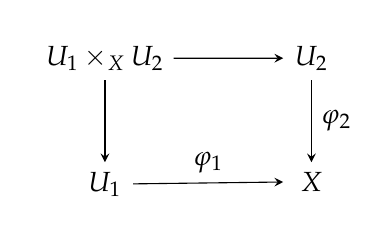
\begin{tikzpicture}
		\matrix (m) [matrix of math nodes,row sep=3em,column sep=4em,minimum width=2em]
		{
			U_1\times_X U_2 & U_2\\ 
			U_1 & X\\};
		\path[-stealth]
		(m-1-1) edge node [above] {} (m-1-2)
		(m-2-1) edge node [above]  {$\varphi_1$} (m-2-2)
		(m-1-1) edge node [right]  {} (m-2-1)
		(m-1-2) edge node [right] {$\varphi_2$} (m-2-2);
	\end{tikzpicture}
	\\
	having the obvious universal property. 
	
\end{definition}
\begin{definition}\label{site_defn}\cite{milne:lec}
	Let  $\mathscr C$  be a category. Suppose that  for each object $U$ of $\mathscr C$ there are  distinguished sets of families of morphisms $\left\{U_\iota \to U\right\}_{\iota\in I}$, called the \textit{coverings} of $U$, 
	satisfying the following axioms: 
	\begin{enumerate}
		\item[(a)] for any covering $\left\{U_\iota \to U\right\}_{\iota\in I}$ and any morphism $U \to V$ in $\mathscr C$, the fibre products 
		$U_\iota\times_U V$ exist, and $\left\{U_\iota\times_U V \to V\right\}_{\iota\in I}$ is a covering of $V$; 
		\item[(b)] if $\left\{U_\iota \to U \right\}_{\iota\in I}$ is a covering of $U$, and if for each $\iota \in I$, $\left\{V_{\iota j} \to U_\iota  \right\}_{j \in I_\iota}$	is a 
		covering of $U_\iota$, then the family $\left\{V_{\iota j }\to U\right\}_{\iota j}$ is a covering of $U$; 
		\item[(c)] for any $U$ in $\mathscr C$, the family $\left\{U\xrightarrow{\Id}U \right\}$ consisting of a single map is a covering of $U$. 
	\end{enumerate}
	The system of coverings is then called a \textit{Grothendieck topology}, and $\mathscr C$  together with 
	the topology is called a \textit{site}. If $\mathbf T$  
	is a site, then $\mathrm{Cat}\left( \mathbf T\right)\bydef \mathscr C$  denotes the underlying category. 
	
\end{definition}
\begin{example}\label{top_gro_exm}
	If $\sX$ is a topological space then one has a category of open subsets and their inclusions. If both $\sU_1, \sU_2 \subset \sX$ are open subsets then one can define a fibre product (cf. Definition \ref{pullback_defn}) by the following way
	$$
	\sU_1\times_\sX \sU_2 \bydef \sU_1 \cap \sU_2.	
	$$
	If $\sU \subset \sX$ is an open subset then we assume that a family  $\left\{\sU_\iota \subset \sU\right\}_{\iota\in I}$, is a covering of $\sU$ (cf. Definition \ref{site_defn}) if and only if  $\sU = \cup_{\iota\in I}\sU_\iota$. This system of coverings is a specialization of Grothendieck topology. 
\end{example}

\begin{definition}\label{top_gro_definition}
	In the situation of the Example \ref{top_gro_exm} one has a site $\mathbf T_{\sX}$ \textit{arising} from $\sX$.
\end{definition}

\begin{definition}\label{etale_presheaf_defn}\cite{milne:lec}
	A \textit{presheaf of sets} on a site $\mathbf T$ 
	is a contravariant functor $\mathscr F$ from $\mathrm{Cat}\left( \mathbf T\right)$ to the category of sets. Thus,  $\mathscr F$
	to each object $U$ in $\mathrm{Cat}\left( \mathbf T\right)$ 
	attaches a set $\mathscr F\left(U \right)$ , and to each morphism $\varphi: U \to V$
	in $\mathrm{Cat}\left( \mathbf T\right)$, a map $\mathscr F\left(\varphi\right):\mathscr F\left(V \right)\to \mathscr F\left(U \right)$. Note that the notion of a presheaf on $\mathbf T$ 
	does not depend on the 
	coverings. We sometimes denote $\mathscr F\left(\varphi\right)$ by $a \mapsto a|_U$.
	
\end{definition}
Similarly, a presheaf of (Abelian) groups or rings on $\mathbf T$ is a contravariant functor from
$\mathrm{Cat}\left( \mathbf T\right)$ to the category of (Abelian) groups or rings.
\begin{definition}\label{etale_sheaf_defn}\cite{milne:lec}
	A \textit{sheaf} on $\mathbf T$ 
	is a presheaf $\mathscr F$ 
	that satisfies the sheaf condition, that is a sequence 
	\be\label{etale_sheaf_eqn}
	\mathscr F \left(U\right) \to \prod_{\iota \in I} \mathscr F \left(U_\iota \right)\rightrightarrows  \prod_{\iota, j \in I\times I} \mathscr F \left(U_\iota \times_U U_j\right)
	\ee
	is exact for every covering $\left\{U_\iota \to U\right\}$. Thus $\mathscr F$ 
	is a sheaf if the map 
	$$
	f \mapsto \left\{f|_{U_\iota }\right\}:\mathscr F \left(U\right) \to \prod_{\iota \in I} \mathscr F \left(U_\iota \right)
	$$
	identifies $\mathscr F\left( U\right)$ with the subset of the product consisting of families $\left\{f_\iota\right\}$ such that 
	$$
	f_\iota|_{U_\iota \times_U U_j}= f_j|_{U_\iota \times_U U_j}
	$$
	for all $\iota, j \in I$. 
	When $\mathbf T$ 
	is the site arising from a topological space then these definitions coincide with the 
	topological ones. 
	
\end{definition}
\begin{definition}\label{forget_sheaf_defn}
	There are categories $\mathbf{PreSh}\left(\mathbf T \right)$, $ \mathbf{Sh}\left(\mathbf T\right)$ of presheaves an sheaves. Moreover there is a \textit{forgetful functor} $\mathfrak{Forget} : \mathbf{Sh}\left(\mathbf T \right)\to \mathbf{PreSh}\left(\mathbf T \right)$.
\end{definition}

\begin{statement}\label{site_sheaf_stmt}\cite{johnstone:topos}
	There is an adjoint $\mathfrak{Ass} : \mathbf{PreSh}\left(\mathbf T  \right)\to \mathbf{Sh}\left(\mathbf T \right)$ to the  forgetful functor $\mathfrak{Forget} : \mathbf{Sh}\left(\mathbf T  \right)\to \mathbf{PreSh}\left(\mathbf T \right)$ (cf. Definition \ref{forget_sheaf_defn}).
\end{statement}	
\begin{defn}\label{site_sheaf_ass_defn}\cite{johnstone:topos}
	The given by the Statement  \ref{site_sheaf_stmt} functor $\mathfrak{Ass} : \mathbf{PreSh}\left(\mathbf T  \right)\to \mathbf{Sh}\left(\mathbf T \right)$  is said to be an  \textit{associated sheaf functor}.
\end{defn}
\begin{statement}\label{site_enough_stmt}\cite{johnstone:topos}
	%8.13$
	If $\mathbf T$ is a site then a category $\mathbf {Ab}\left(\mathbf T \right)$ of sheaves of Abelian groups has enough injectives.
\end{statement}


\begin{definition}\label{constant_presheaf_defn}\cite{johnstone:topos}
	If $X$ is an object of $\mathrm{Cat}\left( \mathbf T\right)$ (cf. Definition \ref{site_defn} then for any set $F$ there is a \textit{constant presheaf} $\mathscr P$ such that $\mathscr P\left( U\right) \bydef F$ and $\mathscr P\left( f\right) \bydef \Id_F$ for all $\mathrm{Cat}\left( \mathbf T\right)/X$-morphism $f: U\to V$.
	We use a following notation
	\be\label{constant_presheaf_eqn}
	F_X \bydef \mathscr P.
	\ee
\end{definition}


If $A$ is a $C^*$-algebra then there is a category $\mathbf{Hered}/A$ such that:
\begin{itemize}
	\item $\mathbf{Hered}/A$-objects are hereditary $C^*$- subalgebras of $A$,
	\item $\mathbf{Hered}/A$-morphism  from $B' \subset A$ to $B'' \subset A$ is a natural inclusion $B'\subset B''$ such that a following diagram 
	\newline
	\begin{tikzpicture}
		\matrix (m) [matrix of math nodes,row sep=3em,column sep=4em,minimum width=2em]
		{
			B'  &  & B''\\ 
			& A &\\};
		\path[-stealth]
		(m-1-1) edge node [above] {$\subset$} (m-1-3)
		(m-1-1) edge node [above]  {} (m-2-2)
		(m-1-3) edge node [right]  {} (m-2-2);
	\end{tikzpicture}
	\\
	is commutative.
\end{itemize}
For any two $\mathbf{Hered}/A$-objects $B', B''$ we define their \textit{fibre product} (cf. Definition \ref{pullback_defn}) by the following way
$$
B'\times_A B'' \bydef B'\cap B''.
$$

\begin{definition}\label{hered_cov_defn}\cite{ivankov:grot_ca}
	For any $\mathbf{Hered}/A$-object $B$ a distinguished set of families of inclusions $\left\{B_\iota \subset B\right\}_{\iota\in I}$, called a \textit{covering} of $B$ if $B$ is a generated by the union $\cup B_\iota$ hereditary $C^*$-subalgebra of $A$ (cf. Definition \ref{hered_gen_defn}).
\end{definition}

\begin{lemma}\label{grothendieck_ca_lem}\cite{ivankov:grot_ca}
	A given by the Definition \ref{hered_cov_defn} system of coverings satisfies to  the Definition \ref{site_defn}, so one has a natural Grothendieck topology.
\end{lemma}



\begin{definition}\label{grothendieck_ca_defn}\cite{ivankov:grot_ca}
	The given by the Lemma \ref{grothendieck_ca_lem} Grothendieck topology  is said to be an  $A$-\textit{topology}. A corresponding  site (cf. Definition \ref{site_defn}) $\mathbf{T}_A$ is said to be \textit{arising} from $A$ (cf. Definition \ref{top_gro_definition}).
\end{definition}


\section{Groupoids, foliations,  and $C^*$-algebras}\label{foliations_sec}
\subsection{Groupoids and their $C^*$-algebras}
\paragraph*{}
A groupoid is a small category with inverses, or more explicitly:
\begin{definition}\label{groupoid_defn}\cite{renault:gropoid_ca}
	% 104
	A \textit{groupoid} consists of a set $\G$, a distinguished subset $\G^0\subset\G$, two maps
	$r, s : \G\to \G^0$ and a law of composition
	$$
	\circ: \G^2\bydef\left\{\left.\left(\ga_1,\ga_2 \right) \in \G\times\G~\right| s\left(\ga_1\right)= r\left(\ga_2\right)\right\}\to \G
	$$
	such that
	\begin{enumerate}
		\item $s\left(\ga_1\circ\ga_2\right)=s\left(\ga_2\right), \quad r\left(\ga_1\circ\ga_2\right)=r\left(\ga_1\right)\quad \forall\left(\ga_1, \ga_2 \right) \in \G$
		\item $s\left(x\right)=r\left(x\right)=x \quad\forall x\in\G^0$
		\item $\ga\circ s\left(\ga\right)= r\left(\ga\right)\circ\ga = \ga\quad \forall\ga\in\G$
		\item $\left( \ga_1\circ\ga_2\right) \circ\ga_3=\ga_1\circ\left( \ga_2\circ\ga_3\right) $
		\item Each $\ga \in\G$ has a two-sided inverse $\ga^{-1}$, with $\ga\circ\ga^{-1}=r\left(\ga\right)$, $\ga^{-1}\circ\ga=r\left(\ga\right)$.
	\end{enumerate}
	The maps $r$, $s$ are called the \textit{range} and \textit{source} maps.
\end{definition}

\begin{definition}\label{groupoid_reduction_defn}\cite{renault:gropoid_ca}
	Let $\G$ be a groupoid, and let $E$ be a subset of $G^0$.
	A subgroupoid 
	$$
	\G^E_E \bydef \left\{x \in G | r(x), s(x)\in E\right\}
	$$
	with unit space $E$ is said to be  the \textit{reduction} 
	of $\G$ by $E$.
\end{definition}
\begin{empt}\cite{renault:gropoid_ca}
	The notion of \textit{topological groupoid} is explained in \cite{renault:gropoid_ca}. 
If $F$ is an Abelian group then then for all $r \ge 0$ there is $r^{\text{th}}$ \textit{cohomology group} $H^r\left( \G, F\right)$. Any element of $H^2\left( \G, F\right)$ can be represented  by a 2-\text{cycle} $\a \in Z^2\left(\G, F \right)$. Note that a 2-cycle $\a$ is a map   $\G^2 \to A$. If $\G$ is a topological groupoid and  $F$ is a topological group then we assume that the map $\a$ is continuous. We write $\left[\a\right]\in H^r\left( \G, F\right)$.
\end{empt}
\begin{remark}\label{hoto_rem}
If both $\a', \a''\in \Z^2\left(\G, F \right)$ a homotopic 2-cocycles  then  $\left[\a'\right]= \left[\a''\right]\in H^2\left( \G, F\right)$.
\end{remark}
\begin{empt}\label{groupoid_haar_empt}\cite{renault:gropoid_ca}
The notion of  \textit{left Haar system} on locally compact groupoid is explained in \cite{renault:gropoid_ca}. Let $\G$ be a locally compact groupoid with left Haar system $\left\{\la^u\right\}$ and let $\a$ be a continuous 2-cocycle in $Z^2\left(\G, \T\right)$. For $f ,g \in C_c(\G )$, let us define
\be\label{groupoid_*_c_eqn}
\begin{split}
	f * g \left(x\right)\bydef 
	\int f ( x y ) g \left( y^{-1}\right)\a\left(xy, y^{-1} \right) d\la^{d(x)}(y),\\
	f^* ( x ) \bydef\overline{f ( x^{ -1})}, 	
\end{split}
\ee	
so $ C_c(\G )$ becomes a *-algebra, we denote it by $C_c\left( \G, \a\right)$. Denote by $C^*_r\left( \G, \a\right)$ a completion of  $C_c\left(\G, \a\right)$ with respect to the following $C^*$-norm
$$
\left\|a \right\| \bydef \sup_{\pi \in \text{Irr}\left(C_c\left(\G\right)\right)} \left\|\pi\left( a\right)  \right\| 
$$
where $\text{Irr}\left(C_c\left(\G\right)\right)$ is a set of all irreducible representations of $C_c\left(\G\right)$.
\end{empt}
\begin{proposition}\cite{renault:gropoid_ca}
	%1.2. Proposition : 
	If $\a$ and $\a'$ are cohomologous, then $C_c\left( \G, \a\right)$  and $C_c\left( \G, \a'\right)$ are
	isomorphic.
\end{proposition}

\subsection{Foliations and pseudogroups}
\begin{definition}\label{foli_trans_defn}\cite{candel:foliI}
	Let $N \subset M$ be a smooth submanifold. We say that $\sF$ is \textit{transverse} to $N$ (and write $\sF\pitchfork N$) if, for each leaf $L$ of $\sF$ and each point $x \in L\cap N$, $T_x\left(L \right)$ ans $T_x\left(N \right)$ together span $T_x\left( M\right)$. At the other extreme At the other extreme, we say that $\sF$ is tangent to $N$ if, for each leaf $L$ of $\sF$, either $L \cap N = \emptyset$ or $L \subset N$.
\end{definition}
The symbol $\mathbb{F}^p$ denotes either the full Euclidean space $\R^p$ or Euclidean half space $\mathbb{H}^p = \left\{\left.\left(x_1,..., x_n \right) \in \mathbb{R}^p\right| x_1 \le 0 \right\}$.
\begin{definition}\label{foli_rect_defn}\cite{candel:foliI}
	A rectangular neighborhood in $\mathbb{F}^n$ is an open subset of the form $B = J_1\times...\times J_n$, where each $J_j$ is a (possibly unbounded) relatively open interval in the $j^{\text{th}}$ coordinate axis. If $J_1$ is of the form $\left( a,0\right]$, we say that $B$ has boundary $\partial B\left\{\left(0, x_2,..., x_n \right)\right\}\subset B$.	%In the following, we will consider coordinate charts that have values in F" x F", allowing the possibility of manifolds with boundary and (convex) COI'Ile1'S.
\end{definition}
\begin{definition}\label{foli_chart_defn}\cite{candel:foliI}
	% 	Definition 1.1.17 \\
	Let $M$ be an $n$-manifold. A \textit{foliated chart} on $M$ of codimension $q$ is a pair $\left(\sU, \varphi)\right)$, where $\sU\subset M$ is open and $\varphi : \sU \xrightarrow{\approx} B_\tau\times B_\pitchfork$ is a diffeomorphism, $B_\pitchfork$ being a rectangular neighborhood in $\mathbb{F}^q$ and $B_\tau$ a rectangular neighborhood in $\mathbb{F}^{n-q}$. The set $P_y = \varphi^{-1}\left(B_\tau \times \left\{y\right\} \right)$ , where $y \in B_\pitchfork$, is called a \textit{plaque} of this foliated chart. For each $x \in B_\tau$, the set  $S_x=\varphi^{-1}\left(\left\{x\right\} \times B_\pitchfork \right)$  is called a \textit{transversal} of the foliated chart. The set $\partial_{\tau}\sU = \varphi^{-1}\left(B_\tau \times \left(\partial B_\pitchfork \right)  \right)$ is called the \textit{tangential boundary} of $\sU$ and $\partial_{\pitchfork}\sU = \varphi^{-1}\left(\partial \left( B_\tau\right)  \times \partial B_\pitchfork \right)$ is called the \textit{transverse boundary} of $\sU$.
\end{definition}

\begin{definition}\label{foli_defn}
	Let $M$ be an $n$-manifold, possibly with boundary and corners, and let $\sF= \left\{L_\la\right\}_{\la \in \La}$ be a decomposition  of $M$ into connected, topologically immersed submanifolds of dimension $k=n-q$. Suppose that $M$ admits an atlas $\left\{\sU_\a \right\}_{\a \in \mathfrak A}$ of foliated charts of codimension $q$ such that, for each $\a \in \mathscr A$ and each $\la \in \La$, $L_\la \cap \sU_\a$ is a union of plaques. Then $\sF$ is said to be a \textit{foliation} of $M$ of codimension $q$ (and dimension $k$) and $\left\{\sU_\a \right\}_{\a \in \mathscr A}$ l is called a \textit{foliated atlas} associated to $\sF$. Each $L_x$ is called a leaf of the foliation and the pair $\left(M, \sF \right)$  is called a \textit{foliated manifold}. If the foliated atlas is of class $C^r$ ($0 \le r \le \infty$ or $r=\om$), then the foliation $\sF$ and the foliated manifold $\left(M, \sF \right)$. is said to be \textit{of class} $C^r$.
\end{definition}
\begin{definition}\label{fol_res_defn}
	If $\left(M,\mathcal F \right)$ is a foliation and $\mathcal{U} \subset M$ be an open subset $\mathcal F|_{\mathcal{U}}$ is the restriction of $\mathcal F$ on ${\mathcal{U}}$ then we say that  $\left(\mathcal{U},\mathcal F|_{\mathcal{U}}\right) $ is the \textit{restriction}   of $\left(M,\mathcal F \right)$ \textit{to}  $\mathcal{U}$. (cf. \cite{connes:ncg94})
\end{definition}
\begin{definition}\label{foli_atlas_defn}
	A \textit{foliated atlas} of codimension $q$ and class $C^r$ on the $n$-manifold $M$ is a $C^r$-atlas $\mathfrak{A}\bydef\left\{\sU_\a \right\}_{\a \in \mathscr A}$  of foliated charts of codimension $q$ which are \textit{coherently foliated} in the sense that, whenever $P$ and $Q$ are plaques in distinct charts of $\mathfrak{A}$, then $P\cap Q$ is open both in $P$ and $Q$. 
\end{definition}
\begin{definition}\label{foli_coh_atlas_defn}
	Two foliated atlases lt and $\mathfrak{A}$ on $\mathfrak{A}'$ of the same codimension and smoothness class $C^r$ are \textit{coherent} ($\mathfrak{A}\approx\mathfrak{A}'$) if $\mathfrak{A}\cup\mathfrak{A}'$ is a foliated $C^*$-atlas.
\end{definition}
\begin{lemma}\label{foli_coh_atlas_eq_lem}
	Coherence of foliated atlases is an equivalence relation.
\end{lemma}
\begin{lemma}\label{foli_coh_atlas_ass_lem}
	Let  $\mathfrak{A}$ and $\mathfrak{A}'$ be foliated atlases on $M$ and suppose that $\mathfrak{A}$ is associated to a foliation $\sF$. Then $\mathfrak{A}$ and $\mathfrak{A}'$ are coherent if and only if $\mathfrak{A}'$ is also associated to $\sF$.
\end{lemma}
\begin{definition}\label{foli_reg_atlas_defn}
	A foliated atlas $\mathfrak{A}\bydef\left\{\sU_\a \right\}_{\a \in \mathscr A}$ of class $C^r$ is said to be \textit{regular} if
	\begin{enumerate}
		\item [(a)] For each $\al \in \mathscr A$, the closure $\overline{\sU}_\al$ of $\sU_\al$ is a compact subset of a foliated chart  $\left\{\sV_\a \right\}$ and $\varphi_\a = \psi|_{\sU_\a }$.
		\item[(b)] The cover $\left\{\sU_\a \right\}$ is locally finite.
		\item[(c)] if $\sU_\a$ and $\sU_\bt$ are elements of $\mathfrak{A}$, then the interior of each closed plaque $P \in \overline \sU_\a$ meets at most one plaque in $\overline \sU_\bt$.
	\end{enumerate}
\end{definition}
\begin{lemma}\label{foli_reg_atlas_ref_lem}
	Every foliated atlas has a coherent refinement that is regular.
\end{lemma}
\begin{thm}\label{foli_thm}
	The correspondence between foliations on $M$ and their associated foliated atlases induces a one-to-one correspondence between the set of foliations on $M$.
\end{thm}

We now have an alternative definition of the term "foliation". 
\begin{defn}\label{foli_alt_defn}
	A \textit{foliation} $\sF$ of codimension $q$ and class $C^r$ on $M$ is a coherence class of foliated atlases of codimension $q$ and class $C^r$ on $M$.
\end{defn}
By Zorn's lemma, it is obvious that every coherence class of foliated atlases contains a unique maximal foliated atlas. 
\begin{defn}\label{foli_max_defn}
	A \textit{foliation of codimension} $q$ and class $C^r$ on $M$ is a maximal foliated $C^r$-atlas of codimension $q$ on $M$.
\end{defn}

\begin{empt}\label{foli_graph_empt}
	Let  $\Pi\left( M,\sF\right)$ be the space of paths on leaves, that is, maps $\a : [0,1] \to M$ that are continuous with respect to the leaf topology on $M$. For such a path  let $s\left(\a \right) = \a\left( 0\right)$  be its source or initial point and let  $r\left(\a \right) = \a\left( 1\right)$ be its range or terminal point. The space $\Pi\left( M,\sF\right)$ has a partially defined multiplication: the product $\a\cdot \bt$ of two elements $\a$ and $\bt$ is defined if the terminal point of $\bt$ is the initial point of $\a$, and the result is the path $\bt$ followed by the path $\a$. (Note that this is the opposite to the usual composition of paths  $\al\#\bt = \bt \cdot \a$ used in defining the fundamental group of a space.)
\end{empt}
\begin{definition}\label{foli_path_space_defn}
	In the situation of \ref{foli_graph_empt} we say that the topological space $\Pi\left( M,\sF\right)$ is the \textit{space of path on leaves}.
\end{definition}
\begin{definition}\label{foli_groupoid_defn}\cite{candel:foliI}
	%Definition 2.3.3.
	A groupoid $\G$ on a set $\sX$ is a category with inverses, having $\sX$ as its set of objects. For $y,z \in \sX$ the set of morphisms of $\G$ from $y$ to $z$ is denoted by $\G^z_y$.
\end{definition}
\begin{defn}\label{foli_graph_defn}\cite{candel:foliII}
	%	Definition 1.3.1
	The \textit{graph}, or \textit{my groupoid}, of the foliated space $\left( M,\sF\right)$  is the quotient space of $\Pi\left( M,\sF\right)$ by the equivalence relation that identifies two paths $\a$ and $\bt$ if they have the same initial and terminal points, and the loop $\a \cdot \bt$ has trivial germinal holonomy.
	The graph of $\left( M,\sF\right)$ will be denoted by $\G\left(M, \sF\right)$, or simply by  $\G\left( M\right)$ or by $\G$ when all other variables are understood.
\end{defn}
\begin{remark}
	There is the natural surjective continuous map
	\be\label{foli_cov_map_eqn}
	\Phi : \Pi\left( M,\sF\right)\to \G\left( M,\sF\right)
	\ee
	from the space of path on leaves to the foliation graph.
\end{remark}
\begin{proposition}\label{foli_chart_prop}
	%	Proposition 1.3.14. \\
	Let $\mathfrak{A}= \left\{\sU_\iota\right\}$ be a regular foliated atlas of $M$. For each finite sequence of indices $\left\{\a_0 ,...,\a_k\right\}$, the product
	\be	\label{foli_chart_eqn}
	\sV_{   \a} =	 \G\left(\sU_{\iota_0} \right)~...~\G\left(\sU_{\iota_k} \right) \in \G\left(M, \sF\right) \quad \a = \left({\iota_0},...,{\iota_k}\right)
	\ee
	is either empty or a foliated chart for the graph $\G$. The collection of all such finite products is a covering of $\G$ by foliated charts. 
\end{proposition}
\begin{theorem}\label{foli_graph_thm}
	The graph $\G$ of $\left( M,\sF\right)$ is a groupoid with unit space $\G_0 = M$, and this algebraic structure is compatible with a foliated structure on $\G$ and $M$. Furthermore, the following properties hold.
	\begin{enumerate}
		\item [(i)] The range and source maps $r, s : \G \to M$ are topological submersions. 
		\item[(ii)] The inclusion of the unit space $M \to\G$ is a smooth map. 
		\item[(iii)] The product map $\G\times_M \G \to G$, given by $\left( \ga_1 , \ga_2\right) \mapsto\ga_1 \cdot \ga_2$, is smooth.
		\item[(iv)]  There is an involution $j: \G \to \G$, given by $j\left( \ga\right) = \ga^{-1}$, which is a diffeomorphism of $\G$, sends each leaf to itself, and exchanges the foliations given by the range. 
	\end{enumerate}
	
\end{theorem}

Above definitions refines the equivalence relation coming from
the partition of $M$ in leaves $M = \cup L_{\alpha}$. 
An element $\gamma$ of $\mathcal G$ is given by two points $x = s(\gamma)$,
$y = r(\gamma)$ of $M$ together with an equivalence class of smooth
paths: $\gamma (t)\in M$, $t \in [0,1]$; $\gamma (0) = x$, $\gamma
(1) = y$, tangent to the bundle $\mathcal{F}$ ( i.e. with $\dot\gamma (t)
\in \mathcal{F}_{\gamma (t)}$, $\forall \, t \in {\mathbb R}$) up to the
following equivalence: $\gamma_1$ and $\gamma_2$ are equivalent if and only if
the {\it my} of the path $\gamma_2 \circ \gamma_1^{-1}$ at the
point $x$ is the {\it identity}. The graph $\mathcal G$ has an obvious
composition law. For $\gamma , \gamma' \in G$, the composition
$\gamma \circ \gamma'$ makes sense if $s(\gamma) = r(\gamma')$. If
the leaf $L$ which contains both $x$ and $y$ has no my, then
the class in $\mathcal G$ of the path $\gamma (t)$ only depends on the pair
$(y,x)$. In general, if one fixes $x = s(\gamma)$, the map from $\mathcal G_x
= \{ \gamma , s(\gamma) = x \}$ to the leaf $L$ through $x$, given
by $\gamma \in \mathcal G_x \mapsto y = r(\gamma)$, is the my covering
of $L$.
Both maps $r$ and $s$ from the manifold $\mathcal G$ to $M$ are smooth
submersions and the map $(r,s)$ to $M \times M$ is an immersion
whose image in $M \times M$ is the (often singular) subset
\begin{equation*}\label{subset}
	\{ (y,x)\in M \times M: \, \text{ $y$ and $x$ are on the same leaf}\}.
\end{equation*}
% We assume, for notational convenience, that the manifold $\mathcal G$ is Hausdorff, but as this fails to be the case in very interesting examples I shall refer to \cite{connes:foli_survey} for the removal of this hypothesis.  
For
$x\in M$ one lets $\Omega_x^{1/2}$ be the one dimensional complex
vector space of maps from the exterior power $\wedge^k \,  \mathcal{F}_x$, $k =
\dim F$, to ${\mathbb C}$ such that
$$
\rho \, (\lambda \, v) = \vert \lambda \vert^{1/2} \, \rho \, (v)
\qquad \forall \, v \in \wedge^k \,  \mathcal{F}_x \, , \quad \forall \,
\lambda \in {\mathbb R} \, .
$$
Then, for $\gamma \in\mathcal G$, one can identify $\Omega_{\gamma}^{1/2}$ with the one
dimensional complex vector space $\Omega_y^{1/2} \otimes
\Omega_x^{1/2}$, where $\gamma : x \to y$. In other words
\be\label{foli_om_g_eqn}
\Omega_{\mathcal G}^{1/2}=\, r^*(\Omega_M^{1/2})\otimes s^*(\Omega_M^{1/2})\,.
\ee

%\begin{empt}\cite{candel:foliI}
%	Page 57.
%The fact that the regular foliated atlas $\mathfrak A$ is locally finite, together with the 2nd countability of $M$, implies that $\mathfrak A$ is at most countably infinite. Thus, the disjoint union 
%\be
%S = \bigsqcup_{\iota \in \I} S_\iota
%\ee	
%is a q-manifold that imbeds as a submanifold $S \hookto M$ is  transverse to $\sF$.
%\end{empt}
%\begin{prdf}\label{foli_preudo_grp_prdf} \cite{candel:foliI}
%	Proposition 2.2.6. I \\
%	Let $\mathfrak{A}$ be a regular foliated atlas of class $C^r$ and let $\ga = \left\{\ga_{\a, \b}\right\}_{\a, \b \in \mathfrak{A}}$ be its my cocycle. Then the set $\Ga_{\mathfrak{A}}$ of my transformations is the $C^r$ pseudogroup on $S$ generated by $\ga$, called the $\mathrm{my~pseudogroup}$ of $\mathfrak{A}$.
%\end{prdf}

\begin{empt}\label{foli_sc_haus_empt}\cite{candel:foliII}
	The  groupoid of a foliated space all leaves of which are simply connected is Hausdorff.
\end{empt}

\begin{exercise}\label{foli_haus_exer}\cite{candel:foliII}
	%: Exercise 1.3.8. 
	Prove or decide the following.
	\begin{enumerate}
		\item The graph of a foliated space all leaves of which are simply connected is Hausdorff.
		\item The graph of a foliated space all leaves of which have trivial holo nomy is Hausdorff.
	\end{enumerate}	
	%	 (1) The graph of a foliated space all leaves of which are simply connected is Hausdorff. (2) The graph of a foliated space all leaves of which have trivial holo nomy is Hausdorff. (3) The graph of the Reeb foliation of the three-sphere is not Hausdorff. (4) True or false: The graph of a codimension one foliated three manifold containing a Reeb component is not Hausdorff.
\end{exercise}



%	\begin{definition}\label{foli_graph_defn1}
	%		The  manifold $\mathcal G$ called the \textit{graph} (or \textit{my groupoid})
	%		of the foliation  $\left(M, \mathcal{F}\right)$  Denote by $\mathcal G\left(M, \mathcal{F}\right)$ the graph of  $\left(M, \mathcal{F}\right)$.
	%	\end{definition}
\begin{definition}\label{foli_pseudo_defn}\cite{candel:foliI}.
	%	Definition 2.2.4. I \\
	Let $N$ be a $q$-manifold. A $C^r$ pseudogroup $\Ga$ on $N$ is a collection of $C^r$ diffeomorphisms $h : D(h) \xrightarrow{\approx} R(h)$ between open subsets of $N$ satisfying the following axioms. 
	\begin{enumerate}
		\item  If $g, h \in \Ga$  and $R(h) \subset G(g)$, then $g \circ h \in \Ga$
		\item	 If $h \in \Ga$, then $h^{-1} \in \Ga$. 
		\item $\Id_N \in \Ga$. 
		\item If $h \in \Ga$ and $W \subset  D(h)$ is an open subset, then $\left.h\right|_W \in \Ga$. 
		\item If $h:D(h) \xrightarrow{\approx} R(h)$ is a $C^r$ diffeomorphism between open subsets of $N$ and if, for each $w \in  D(h)$, there is a neighborhood $W$ of $w\in  D(h)$ such that $\left.h\right|_W \in \Ga$, then $h \in \Ga$. 
	\end{enumerate}
	If $\Ga' \subset \Ga$ is also a pseudogroup, it is called a subpseudogroup of $\Ga$.
\end{definition}

\begin{remark}
	Any pseudogroup is a groupoid (cf. Definition \ref{groupoid_defn}).
\end{remark}
\begin{remark}\cite{candel:foliI}\label{foli_pseudo_rem}
	In the case of general foliations, the total my group of a foliated bun dle must be replaced by a local analogue called the \textit{my pseudogroup}.
\end{remark}
\begin{remark}\label{foli_groupoid_n_red_defn}
	If $\left(M, \sF\right)$ is a foliated manifold and $N$ is a tranversal then
	\be\label{foli_gnn_eqn}
	\G^N_N \bydef \left\{\left. \ga \in \G\left(M, \sF\right)\right| s\left(\ga\right), r\left(\ga\right)\in N\right\}
	\ee
	is	a pseudogroup. 
	
	
\end{remark}
\begin{definition}
	In the above situation we say that $\G^N_N$ is a \textit{reduced groupoid}.
\end{definition}

\subsection{Operator algebras of foliations}\label{foli_alg_subsec}
\paragraph*{}
Here I follow to \cite{candel:foliII,connes:ncg94}.  Since the bundle $\Om^{1/2}$ is trivial (because $\G\left(M, \sF\right)$ admits partitions of unity), a choice of an everywhere positive density $\nu$ allows us to identify $\Ga_c\left(\G\left(M, \sF\right),\Om^{1/2}  \right)$  with $\Coo_c\left( \G\left(M, \sF\right)\right)$. 
The definition of foliated space makes sense even when the underlying topological space fails to satisfy the Hausdorff separation axiom. Non-Hausdorff spaces appear naturally in the theory of foliations. In a graph of a foliated space is not necessary Hausdorff. It will be necessary to use functions with compact support on such spaces. However, a non-Hausdorff space may not have sufficiently many such functions, the basic reason being that compact subsets of a Hausdorff space are not necessarily closed. The non-Hausdorff spaces that will appear here have a particularly simple local structure, and even when it is possible to construct appropriate functions using this local structure, the standard operation of ?extension by 0� of local objects to the full space does not pro duce continuous functions. M. Crainic and I. Moerdijk \cite{cra_moe:nhaus} proposed a very natural way of dealing with this problem, and this preliminary section describes it. (That paper develops an extended sheaf  theory for non-Hausdorff manifolds (cf. Appendix \ref{sheaves_nh_sec})).
Here $\sX$ will denote a separable topological space having the structure of a foliated space, but it is not required that the topology be Hausdorff. It is only required that $\sX$ can be covered by countably many open sets homeomorphic to a product $\D \times \mathcal Z$, where $D$ is an open ball in Euclidean $n$-space and $\mathcal Z$ is a separable locally compact Hausdorff space. Let $\mathcal C\infty$ denote the structure sheaf  of the foliated space $\sX$, that is, the sheaf  of smooth functions on $\sX$. Let $\A$ be a sheaf of $\mathcal C\infty$-modules over $\sX$, for instance, the sheaf  of differential forms or other sheaves of smooth sections of foliated vector bundles. For such a sheaf  $\A$ over $\sX$, let $\A$ denote its Godement resolution: $A'\left(\sU\right)$ is the set of all sections (continuous or not) of $\A$ over $\sU\subset\sX$. For a Hausdorff open subset $\mathcal W$ of $\sX$, let $\Ga_c\left( \mathcal W, \A\right) $ denote the set of continuous compactly supported sections of $\A$ over $\mathcal W$. If $\mathcal W\subset\sU$, then ?extension by 0� induces a well defined homomorphism $\Ga_c\left( \mathcal W, \A\right)\to \A'\left(\sU \right)$. For an open subset $\sU$ of $\sX$, let $\Ga_c\left( \mathcal U, \A\right)$ denote the image of the homomorphism $\oplus \Ga_c\left( \mathcal W, \A\right)\to \A'\left(\sU\right)$ (cf. Definition \ref{nh_csoft_gc_defn}). From the equation \eqref{sheaf_inc_eqn} it follows that there is the inclusion
\be\label{foli_incc_eqn}
\Ga_c\left(\mathcal W, \A \right) \hookto \Ga_c\left(\mathcal U, \A \right).
\ee
Let $\G\bydef \G\left(M, \sF \right)$ be a foliation chart. 	The bundle $\Omega_M^{1/2}$ is trivial on $M$, and we
could choose once and for all  a trivialisation $\nu$ turning
elements of $\Ga_c \left(\mathcal G , \Omega_{\mathcal G}^{1/2}\right)$ into functions.
Let us
however stress that the usage of half densities makes all the
construction completely canonical.
For $f,g \in \Ga_c \left(\mathcal G , \Omega_{\mathcal G}^{1/2}\right)$, the convolution
product $f * g$ is defined by the equality
\be\label{foli_prod_eqn}
(f * g) (\gamma) = \int_{\gamma_1 \circ \gamma_2 = \gamma}
f(\gamma_1) \, g(\gamma_2) \, .
\ee
This makes sense because, for fixed $\gamma : x \to y$ and fixing $v_x
\in \wedge^k \,  \mathcal{F}_x$ and $v_y \in \wedge^k \,  \mathcal{F}_y$, the product
$f(\gamma_1) \, g(\gamma_1^{-1} \gamma)$ defines a $1$-density on
$G^y = \{ \gamma_1 \in G , \, r (\gamma_1) = y \}$, which is smooth
with compact support (it vanishes if $\gamma_1 \notin\supp f$),
and hence can be integrated over $G^y$ to give a scalar, namely $(f * g)
(\gamma)$ evaluated on $v_x , v_y$.
The $*$ operation is defined by $f^* (\gamma) =
\overline{f(\gamma^{-1})}$,  i.e. if $\gamma : x \to y$ and
$v_x \in \wedge^k \, \mathcal{F}_x$, $v_y \in \wedge^k \, \mathcal{F}_y$ then $f^*
(\gamma)$ evaluated on $v_x , v_y$ is equal to
$\overline{f(\gamma^{-1})}$ evaluated on $v_y , v_x$. We thus get a
$*$-algebra $\Ga_c \left(\mathcal G , \Omega_{\mathcal G}^{1/2}\right)$. 
where $\xi$ is a square integrable half density on $\mathcal G_x$. 
For each leaf $L$ of
$\left(M, \mathcal{F}\right)$ one has a natural representation of this $*$-algebra on the
$L^2$ space of the my covering $\tilde L$ of $L$. Fixing a
base point $x \in L$, one identifies $\tilde L$ with $\mathcal G_x = \{
\gamma , s(\gamma) = x \}$ and defines
\begin{equation}\label{foli_repr_eqn}
	(\rho_x (f) \, \xi) \, (\gamma) = \int_{\gamma_1 \circ \gamma_2 =
		\gamma} f(\gamma_1) \, \xi (\gamma_2) \qquad \forall \, \xi \in L^2
	(\mathcal G_x),\
\end{equation}


Given
$\gamma : x \to y$ one has a natural isometry of $L^2 (\mathcal G_x)$ on $L^2
(G_y)$ which transforms the representation $\rho_x$ in $\rho_y$.
\begin{lemma}
	%	Lemma 1.4.1. \\
	If $f_1 \in \Ga_c\left(\sU_{   \a_1},\Om^{1/2} \right)$ and $f_2 \in \Ga_c\left(\sU_{   \a_2},\Om^{1/2} \right)$ then their convolution is a well-defined element $f_1*f_2 \in \Ga_c\left(\sU_{   \a_1}\cdot\sU_{   \a_2},\Om^{1/2} \right)$
\end{lemma}
%page 24.
%Let $\Ga_c\left( \G,\Om^{1/2}\right)$  be the space of compactly supported smooth sections of $\Om^{1/2}$ over $\G$; its elements are the compactly supported half-densities on G. When G is not Hausdorff, the meaning of c (G,D1/2) is that which was described in Section 1.2. This space will now be given the structure of an algebra with involution. This structure is first described when G is Hausdorff, and the details will then be given when G is arbitrary.

\begin{proposition}\label{foli_repr_prop}
	%Proposition 1.4.5. \\
	If $\sV \subset \G$ is a foliated chart for the graph of $\left(M, \sF\right)$ and $f \in \Ga_c\left(\sV, \Om^{1/2}\right)$ , then $\rho_x\left( f\right)$, given by \eqref{foli_repr_eqn}, is a bounded integral operator on $L^2\left(\G_x \right)$.
\end{proposition}
\begin{empt}
	The space of compactly supported half-densities on $\G$ is taken as given by the exact sequence 
	\be\label{foli_ga_p_eqn}
	\bigoplus_{\a_0\a_1}\Ga_c\left(\sU_{   \a_0\a_1}, \Om^{1/2} \right) \to \bigoplus_{\a_0}\Ga_c\left(\sU_{   \a_0},\Om^{1/2} \right) \xrightarrow{\Ga_\oplus}  \Ga_c\left(\G,\Om^{1/2}\right) 
	\ee
	associated to a regular cover for $\left((M, \sF)\right)$ as above. The first step for defining a convolution is to do it at the level of $\bigoplus_{\a_0}\Ga_c\left(\sU_{   \a_0}\Om^{1/2} \right)$, as the following lemma indicates. 
\end{empt}




\begin{defn}\label{foli_red_defn}
	% 	Definition 1.4.7.\\
	The \textit{reduced} $C^*$-algebra of the foliated space $\left(M,\sF\right)$ is the completion of $\Ga_c\left( \G,\Om^{1/2}\right)$ with respect to the pseudonorm \be\label{foli_pseudo_norm_eqn}
	\left\|f \right\| =\sup_{x \in M}\left\|  \rho_x\left(f\right)\right\|
	\ee where $\rho_x$ is given by  \eqref{foli_repr_eqn}.
	This $C^*$-algebra is denoted by $C^*_r\left(M,\sF\right)$.
\end{defn} 
An obvious consequence of the construction of 
$C^*_r\left(M,\sF\right)$ is the following. 

\begin{cor}\label{foli_cov_alg_cor}
	%	Corollary 1.4.8.
	Let $M$ be a foliated space and let $\mathfrak{A}$ be a regular cover by foliated charts. Then the algebra generated by the convolution algebras $\Ga_c\left( \G\left(\sU \right), \Om^{1/2}\right)$, $~\sU\in\mathfrak{A}$ is dense in  $C^*_r\left(M,\sF\right)$.
\end{cor}
\begin{empt}\label{foli_res_inc_empt}
	%	page 29-30.
	Let $\left(M,\sF\right)$ be an arbitrary foliated space and let $\sU\subset  M$ be an open subset.  Then $\left(\sU,\sF|_\sU\right)$ is a foliated space and the inclusion  $\sU\hookto  M$ induces a homomorphism of groupoids $\G\left(\sU \right)\hookto \G$ , hence a mapping
	\be\label{foli_inc_gc_eqn}
	j_\sU : \Ga_c\left(  \G\left(\sU \right) ,\Om^{1/2}\right)  \hookto \Ga_c\left( \G\left( M\right) ,\Om^{1/2}\right)
	\ee
	that is an injective homomorphism of involutive algebras. 
	%	It is proven in \cite{candel:foliII,connes:foli_survey} that any restriction of foliation induces an injective *-homomorphism 
	%	\begin{equation}\label{fol_res_hom_eqn}
		%	C^*_r\left(\mathcal{U},\mathcal F|_{\mathcal{U}} \right)\hookto C^*_r\left(M,\mathcal F \right).
		%	\end{equation}
\end{empt}
\begin{prop}\label{foli_res_inc_prop} %	Proposition 1.5.5. 
	Let $\sU$ be an open subset of the foliated space $M$. Then the inclusion $\sU \hookto M$ induces an isometry of $C^*_r\left(\sU,\sF|_\sU\right)$  into $C^*_r\left(M,\sF\right)$.
\end{prop}
\begin{lemma}\label{foli_leaf_lem}
	%Lemma 1.4.9. 
	Each element $\ga \in \G$ induces a unitary operator $\rho_\ga : L^2\left(s\left( \ga\right)\right)   \xrightarrow{\approx}  L^2\left(r\left( \ga\right)\right) $   that conjugates the operators $\rho_{s\left(\ga \right)} \left(f \right) $ and $\rho_{r\left(\ga \right)} \left(f \right)$. In particular, the norm of $\rho_x\left(f \right)$  is independent of the point in the leaf through $x$.
\end{lemma}

\begin{lem}\label{foli_point_lem}
	%Lemma 1.4.10. 
	If $f \in \Ga^\infty_c\left(\G, \Om^{1/2}\right)$ does not evaluate to zero at each $\ga \in \G$, then there exists a point $x$ in $M$ such that $\rho_x\left( f\right)  \neq  0$.
\end{lem}
%\begin{defn} \label{foli_full_defn} NECESSARY
%  Definition 1.4.12. The full $C^*$-algebra of the foliated space $\left(M, \sF\right)$ denoted by $C^*_r\left(M, \sF\right)$, is the completion of %c(G,D1/2) with respect to the pseudonorm f=f= sup?(f), where runs through all the involutive representations of c (G,D1/2) on a separable Hilbert space whose restrictions to the graph G(U) of each foliated chart U for (M,F) are weakly continuous for the inductive limit ... Because each Rx, x  M, is an involutive representation of the convolution 
%\end{defn}
\begin{definition}\label{foli_fibration_defn}\cite{candel:foliI}
	A foliated space $\left(M, \sF\right)$ is a \textit{fibration} if for any $x$ there is an open transversal $N$ such that $x\in N$ and for every  leaf $L$ of $\left(M, \sF\right)$ the intersection $L\cap  N$ contains no more then one point.
\end{definition}
\begin{prop}\label{foli_one_leaf_prop}
	% Proposition 1.5.1. 
	The reduced $C^*$-algebra of a foliated space $M$ consisting of exactly one leaf is the algebra $\K\left( L^2\left(M \right) \right)$  of compact operators on $L^2\left(M \right)$.
\end{prop}


\begin{prop}\label{foli_tens_comp_prop}\cite{candel:foliII}
	% Proposition 1.5.4. \\
	The reduced  $C^*$-algebra $C^*_r\left(\mathcal N\times \mathcal Z \right)$ of the trivial foliated space $\mathcal N \times \mathcal Z$ is the tensor product $\K\otimes C_0\left(\mathcal Z\right)$, where $\K$ is the algebra of compact operators on $L^2\left(\mathcal N \right)$  and $ C_0\left(\mathcal Z\right)$ is the space of continuous functions on $\mathcal Z$ that vanish at infinity.
\end{prop}
\begin{thm}\label{foli_tens_comp_thm}\cite{candel:foliII}
	%	Theorem 1.5.12. 
	Assume that $\left(M, \sF\right)$ is given by the fibers of a fibration $p : M \to B$ with fiber $F$. Then $\left(M, \sF\right)$ is isomorphic to $C_0\left(B\right)\otimes \K\left(L^2\left(N\right)\right)$.
\end{thm}
\begin{remark}\label{foli_x_state_rem}
	It is proven in \cite{candel:foliII} (See Claim 2, page 56) that for any $x \in M$ the given by \eqref{foli_repr_eqn} representation $\rho_x: C^*_r\left(M, \sF \right)\to B\left( L^2\left(\G_x \right)\right)$   corresponds to a state $\tau_x : C^*_r\left(M, \sF \right)\to \C$.
\end{remark}



%\begin{definition}\label{foli_pseudo_a_defn}\cite{candel:foliII}
%Definition 1.3.6.\\ 
%The my pseudogroup of a foliated space is \textit{pseudo analytic} if the following holds. If $h: Z\to Z'$ is a my transformation between two transversals $Z$ and $Z'$, with $Z\subset Z'$, and $W \subset Z$ is an open subset such that $\left.h\right|_W = \Id$, and if $x \in \overline{W}$ is such that $h(x) = x$, then $h = \Id$ on a neighborhood of x. 
%\end{definition}

%\begin{proposition}\label{foli_pseudo_a_prop}\cite{candel:foliII}
%Proposition 1.3.7. \\
%Let M be a foliated space. Then the graph of M is Hausdorff if and only if the my pseudogroup of M is pseudo-analytic.
%\end{proposition}
\begin{theorem}\label{foli_irred_hol_thm}\cite{candel:foliII}
	%Theorem 1.4.11. 
	Let $(M,\sF)$ be a foliated space and let $x \in M$. Then the representation $\rho_x$ is irreducible if and only if the leaf through $x$ has no holonomy.
\end{theorem}
\begin{empt}\label{foli_pseudo_empt}\cite{connes:ncg94}
	%Page 126 
	If $\G^N_N$ is a  given by \eqref{foli_gnn_eqn} pseudogroup then $\G^N_N$ is a manifold.  One can define a structure of $*$-algebra on $\Coo_c\left( \G^N_N\right)$ such that for any $a, b \in \Coo_c\left( \G^N_N\right)$ one has:
	\be\label{foli_pseudo_eqn}
	\begin{split}
		\left(a\cdot b\right)\left(\ga\right)= \sum_{\ga_1\circ\ga_2=\ga}a\left( \ga_1\right)a\left( \ga_1\right),\\
		a^*\left(\ga\right)= \overline{a\left(\ga^{-1}\right)} 
	\end{split}
	\ee
	Denote by $C^*_r\left(	\G^N_N \right)$ the reduced algebra of $\G^N_N$ (cf. Definition \ref{foli_groupoid_red_defn}). The equation \eqref{foli_pseudo_eqn} is a specialization of the \eqref{groupoid_a_eqn} one. 
\end{empt} 	

\begin{theorem}\label{foli_mor_thm}\cite{candel:foliII}
	%Theorem 1.5.16. 
	Let $(M,\F)$ be a foliated space and let $(Z, \mathscr H)$ be the holonomy pseudogroup associated to a complete transversal $Z$. Then the foliation $C^*$-algebra is Morita equivalent to the pseudogroup $C^*$-algebra.
\end{theorem}
\begin{remark}\label{foli_comp_trans_rem}
	A transversal is \textit{complete} if it meets any leaf.
\end{remark}
\begin{remark}\label{foli_pseudo_alg_rem}
	A pseudogroup $C^*$-algebra is $C^*_r\left(	\G^N_N \right)$.
\end{remark}


%\begin{lemma}
%	Il existe un recouvrement distingu�  localement  	fini de $V$ par des ouverts trivialisants $\Om_j$, $j \in \left\{1, 2,. . . , n, . . .\right\}$ et  	des transversales $T_j$, dans $\Om_j$ tels que les adh�rences $\overline T_j$, dans $V$ des  	$T_j$ soient deux ? deux disjointes. 
%	\end{lemma}
The following  lemma is a more strong version of the Theorem \ref{foli_mor_thm}.
\begin{lemma}\label{foli_stab_lem}\cite{hilsum_scandalis:stab}
Si $N$ est une transversale fid�le de $M$
on a: $C^*_r\left(M, \sF \right)\cong C^*_r\left(\G^N_N \right)\otimes \K$.
\end{lemma}
\begin{remark}\label{foli_stab_rem}
The English translation of the Theorem \ref{foli_stab_lem} is "if $N$ is a complete transversal then $C^*_r\left(M, \sF \right)\cong C^*_r\left(\G^N_N \right)\otimes \K$".
\end{remark}
\begin{empt}\label{foli_stab_empt}
Besides the Lemma \ref{foli_stab_lem} we need some details of its proof. If $N$ is a complete transversal and
$$
E^M_N \bydef \Ga_c\left(r^{-1}\left(M \right), s^*\left(\Om^{1/2} \right)   \right) 
$$
then there is a $\Ga_c\left(\G, \Om \right)$-valued product  on $E^M_N$ given by
$$
\left\langle \xi, \eta \right\rangle\left( \ga\right) = \sum_{\substack{ s\left(\ga\right)=s\left(\ga'\right)\\r\left(\ga'\right)\in N}}\overline\xi\left(\ga'\circ\ga^{-1}\right)\eta\left(\ga'\right), \quad %\forall \xi,\eta\in \Ga_c\left(r^{-1}\left(M \right), s^*\left(\Om^{1/2} \right).
$$
If $\E^M_N$ is a completion of $E^M_N$ with respect to the norm $\left\| \xi\right|  \bydef \sqrt{\left\langle \xi, \xi \right\rangle}$ then $\E^M_N$ is $C^*_r\left(M,\sF\right)$-$C^*_r\left(\G^N_N\right)$-imprimitivity bimodule. (cf. Definition \ref{strong_morita_defn}). It follows that
\be\label{foli_k1_eqn}
C^*_r\left(M,\sF\right)\cong \K\left(\E^M_N\right).
\ee
On the other hand in \cite{hilsum_scandalis:stab} it is proven that there is an isomorphism 
\be\label{foli_k2_eqn}
\E^M_N\cong\ell^2\left(C^*_r\left(\G^N_N\right) \right)\cong C^*_r\left(\G^N_N\right)\otimes \ell^2\left( \N\right).  
\ee
The combination of equations \eqref{foli_k1_eqn}, \eqref{foli_k2_eqn} yields the Lemma  \ref{foli_stab_lem}.
Below we briefly remind  the idea described in \cite{hilsum_scandalis:stab} proof of the equation  \ref{foli_k2_eqn}. There is a tubular neighborhood $V_N$ of $N$ which is homeomorphic to $N \times [0,1]^q$. This neighborhood yields the isomorphism
\be\label{foli_e_sum_eqn}
\E^M_N\cong C^*_r\left(\G^N_N\right)\otimes L^2\left( [0,1]^q\right) \oplus  \E^W_N
\ee
where $\E^W_N$ is a countably generated Hilbert $C^*_r\left(\G^N_N\right)$-module.
From $ L^2\left( [0,1]^q\right)\cong\ell^2\left(\N\right)$ and the Kasparov stabilization theorem \ref{kasparov_stab_thm}, it follows that\\ $\E^M_N\cong\ell^2\left(C^*_r\left(\G^N_N\right) \right)$. If we  select any
\be\label{foli_vec_eqn}
\xi \in L^2\left( [0,1]^q\right)
\ee
such that $\left\|\xi\right\|= 1$ then  is an orthogonal basis
\be\label{foli_basis_eqn}
\left\{\eta_j\right\}_{j\in \N}\subset \ell^2\left(\N \right), \quad\eta_1\bydef\xi
\ee
In this basis the element  $a\otimes \xi\left\rangle \right\langle \xi\in C^*_r\left(\G^N_N\right)\otimes \K$ is represented by the following matrix
\be\label{foli_mat_eqn}
a\otimes \xi\left\rangle \right\langle \xi  =  	\begin{pmatrix}
	a& 0 &\ldots \\
	0& 0 &\ldots \\
	\vdots& \vdots &\ddots\\
\end{pmatrix}.
\ee

\end{empt}
\begin{theorem}\cite{candel:foliII}
%	Theorem 1.5.16. 


Let $(M, \sF)$ be a foliated space and let $\left(Z, \mathcal H\right)$ be the holonomy
pseudogroup associated to a complete transversal $Z$. Then the foliation
$C^*$-algebra is Morita equivalent to the pseudogroup $C^*$-algebra.
\end{theorem}	
\begin{example}\label{fol_tor_exm}\emph{Linear foliation on torus.} Here I follow to \cite{connes:ncg94}.
Consider a vector field $\tilde{X}$ on $\R^2$ given by
\[
\tilde{X}=\alpha\frac{\partial}{\partial
	x}+\beta\frac{\partial}{\partial y}
\]
with constant $\alpha$ and $\beta $. Since $\tilde{X}$ is
invariant under all translations, it determines a vector field $X$
on the two-dimensional torus ${\T}^2={\R}^2/{\Z}^2$. The vector
field $X$ determines a foliation $\mathcal{F}$ on ${\T}^2$. The leaves of
$\mathcal{F}$ are the images of the parallel lines
$\tilde{L}=\{(x_0+t\alpha, y_0+t\beta): t\in\R\}$ with the slope
$\theta=\beta/\alpha $ under the projection $\R^2\to \T^2$.
In the case when $\theta$ is rational, all leaves of $\mathcal{F}$ are
closed and are circles, and the foliation $\mathcal{F}$ is determined by
the fibers of a fibration $\T^2\to S^1$. In the case when $\theta$
is irrational, all leaves of $\mathcal{F}$ are everywhere dense in $\T^2$. We say that  $\left(\T^2, \mathcal{F}_\th \right)$ is  the \textit{Kronecker foliation} $dy = \th dx$ of the 2-torus $ \T^2 \bydef \R^2/\Z^2$ 
with natural coordinates $\left((x, y \right)\in \R^2$. Here $\th\in (0,1)$ is an irrational number.
The graph $\G$ of this foliation is the manifold $\G \cong \T\times \R$ with range and source maps  $\G \to \T^2$ given by
\bean
r((x, y), t) = (x + t, y + \th t).\\
s((x, y), t) = (x, y)
\eean
and with composition given by $((x, y), t)((x_0, y_0), t_0) = ((x_0, y_0), t + t_0)$ for any pair of	composable elements.
Every closed geodesic of the at torus $\T^2$ yields a compact transversal. More precisely,
for each pair $(p, q)$ of relatively prime integers we let $N_{p,q}$ be the submanifold of $\T^2$
given by
$$
N_{p,q} = \left\{(ps, qs) | s\in \R/\Z\right\}
$$
The graph $\G$ reduced by $N = N_{p,q}$, i.e. $\G^N_N \bydef \left\{\left.\ga \in \G \right| r(\ga)\in N, \quad s(\ga)\in N\right\}$
the manifold $\G^N_N=\T\times \Z$ with range and source maps given by:
\bean
r(x, n) = x + n\th' ;\\
s(x, n) = x
\eean
where $\th'$ is determined uniquely by any pair $(p_0, q_0)$ of integers such that $pq_0 - p_0q= 1$, $\quad \th' = \frac{p'\th - q'}{p\th - q}$
%	The $C^*$-algebra $C^*_{r,N}\left( \T^2, F\right)$ 
%	is the crossed product of $C(\T)$ by the rotation of angle $\th'$,
%	i.e. it is the irrational rotation $C^*$-algebra $C\left(\T_{\th'}\right)$, generated by two unitaries $U$
%	and $V$ such that:
%	$$
%	VU = e^{2\pi i\th' } UV,
%	$$
%	Since $N = N_{p,q}$ meets every leaf 
%	of the foliation, it follows that $C^*_r (V, F)$ is strongly
%	Morita equivalent to $C\left(\T_{\th'}\right)$ for any relatively prime pair $(p, q)$. In particular for $p = 0,~
%	q = 1$ we get $C\left(\T_{\th}\right)$, and, by transitivity of strong Morita equivalence
If $N = N_{0,1}$ then 
\bean
r(x, n) = x + n\th ;\\
s(x, n) = x
\eean
Let $U$ be an element of $C\left(\T\right)$ which comes from
\bean
U:\R \to \C,\\
t \mapsto e^{2\pi i t}.
\eean
If both  $u, v\in C^\infty_c\left(\G^N_N \right)$ are such that
\be\label{foli_uv_eqn}
\begin{split}
	u\left(x, n \right) = \begin{cases}
		U\left(x \right) & n = 0\\
		0 & n\neq 0
	\end{cases};\\
	v\left(x, n \right) = \begin{cases}
		1 & n = 1\\
		0 & n\neq 1
	\end{cases},\\
\end{split}
\ee
then from  the equations \eqref{foli_pseudo_eqn}
one has
\bean
u^*=u^{-1},\\
v^*=v^{-1},\\
vu = e^{2\pi i\th } uv.
\eean
Indeed above equations describe a noncommutative 2-torus $C\left(\T^2_\th\right)$ (cf Definition \ref{nt_defn}). Using this fact one deduce that 
\be\label{foli_nt_eqn}
C^*_r\left( \G^N_N\right) \cong C\left(\T^2_\th\right).
\ee
\end{example}



\subsection{Restriction of foliation}


\begin{lemma}\label{fol_res_lem}\cite{connes:ncg94}
If $\sU \subset M$ is an open set and  $\left(\mathcal{U},\mathcal F|_{\mathcal{U}}\right) $ is the {restriction}   of $\left(M,\mathcal F \right)$ {to}  $\mathcal{U}$ then the graph 
$\G\left(\mathcal{U},\mathcal F|_{\mathcal{U}}\right)$ is an open set in the graph $\G\left(M,\mathcal F \right)$, and the inclusion
$$
\Coo\left(\mathcal{U},\mathcal F|_{\mathcal{U}}\right)\hookto\Coo\left(M,\mathcal F \right)
$$
extends to an isometric *-homomorphism of $C^*$-algebras
$$
C^*_r\left(\mathcal{U},\mathcal F|_{\mathcal{U}}\right)\hookto C^*_r\left(M,\mathcal F \right).
$$
\end{lemma}

\begin{remark}\label{fol_res_rem}\cite{connes:ncg94}
This lemma, which is still valid in the non-Hausdorff case \cite{connes:foli_survey}, allows one to reflect
algebraically the local triviality of the foliation.
Thus one can cover the manifold $M$ by
open sets $\sU_\la$ such that $\sF$ restricted to $\sU_\la$ has a Hausdorff space of leaves, $\sV_{\la} = \sU_\la/\sF$. and hence such that the C*-algebras $C^*_r\left(\mathcal{U}_\la,\mathcal F|_{\mathcal{U}_\la}\right)$  are strongly Morita equivalent to the commutative $C^*$-algebras $C_0\left( B_\la\right)$. These subalgebras $C^*$-algebras $C^*_r\left(\mathcal{U}_\la,\mathcal F|_{\mathcal{U}_\la}\right)$ generate $ C^*_r\left(M,\mathcal F \right)$. 
but of course they fit together in a very complicated way which is related to the global
properties of the foliation.
\end{remark}
\end{appendices}
			
%\section*{Acknowledgment}


%\paragraph*{}
% I am grateful to my grandfather Petr who forested my mind and my grandson Petr who  watched my work.
 

 
 \begin{thebibliography}{10}
 	


%\bibitem{godement:sheaf} Roger Godement, \textit{Topologie Alg�brique et Th�orie des Faisceaux}. Actualit�s Sci. Ind. No. 1252. Publ. Math. Univ. Strasbourg. No. 13 Hermann, Paris. 1958.

%\bibitem{goldblatt:topoi} Robert Goldblatt. \textit{Topoi: The Categorial Analysis of Logic}. Revised edition of XLVII 445. Studies in logic and the foundations of mathematics, vol. 98. North-Holland, Amsterdam, New York, and Oxford, 1984, xvi + 551 pp. 1984.
\bibitem{bryl:loop}Jean-Luc Brylinski. \textit{Loop Spaces, Characteristic Classes and Geometric Quantization}. Springer Science \& Business Media, Nov 15, 2007.
\bibitem{candel:foliI}Alberto Candel, Lawrence Conlon. \textit{Foliations I}. Graduate Studies in Mathematics, American Mathematical Society (1999), 1999.


\bibitem{candel:foliII}Alberto Candel, Lawrence Conlon. \textit{Foliations II}. American Mathematical Society; 1 edition (April 1 2003), 2003.
\bibitem{cuntz_meyer_ros:bivariant} Joachim Cuntz, Ralf Meyer, Jonathan M. Rosenberg.
\textit{Topological and Bivariant K-Theory}. (Oberwolfach Seminars, 36, Band 36) 2010.
\bibitem{eust} Samuel Eilenberg, Norman E. Steenrod, \textit{Foundations of Algebraic Topology}. Published by Princeton University Press 1952.
%\bibitem{dimca:sheaves} Alexandru Dimca. \textit{Sheaves in Topology} Springer Science \& Business Media, Mar 12, 2004. 

\bibitem{engelking:general_topology} Ryszard Engelking. \textit{General topology}, PWN, Warsaw. 1977.

\bibitem{ivankov:grot_ca}Petr R. Ivankov. \textit{Grothendieck topology of $C^*$-algebras}, arXiv:2306.14684, 2023.

%\bibitem{gelfand_manin} Sergei I. Gelfand, Yuri I. Manin. \textit{Methods of Homological Algebra},  Springer Monographs in Mathematics (SMM), 1996.

\bibitem{hartshorne:ag} Robin Hartshorne. {\it Algebraic Geometry.} Graduate Texts in Mathematics, Volume 52, 1977.

\bibitem{matro:hcm} Manuilov V.M., Troitsky E.V. \textit{Hilbert $C^*$-modules}. % Publication Year: 2005. ISBN-10: 0-8218-3810-5 ISBN-13: 978-0-8218-3810-5 
Translations of Mathematical Monographs, vol. 226, 2005.

\bibitem{milne:lec} J.S. Milne. \textit{Lectures on \'Etale Cohomology}. Version 2.21 March 22, 2013.

\bibitem{murphy}G.J. Murphy. {\it $C^*$-Algebras and Operator Theory.} Academic Press 1990.



\bibitem{johnstone:topos}P.T. Johnstone. \textit{Topos Theory}, L. M. S. Monographs no. 10, Academic Press 1977.

\bibitem{pedersen:ca_aut}Gert Kj�rg�rd Pedersen. {\it $C^*$-algebras and their automorphism groups}. London ; New York : Academic Press, 1979.

\bibitem{rae:ctr_morita} Iain Raeburn, Dana P. Williams. \textit{Morita Equivalence and Continuous-trace $C^*$-algebras}. American Mathematical Soc., 1998.

\bibitem{renault:gropoid_ca} Jean Renault, \emph{A groupoid approach to {$C\sp{\ast} $}-algebras}, Lecture Notes in Mathematics, vol. 793, Springer, Berlin, 1980. 



\end{thebibliography}




 \end{document}


